\chapter{The Balloon Experimental Twin Telescope for Infrared Interferometry}
\label{chap:BETTII}

\section{Towards higher angular resolution in the far-IR}
Observations at mid- to far-infrared wavelengths from the Earth's surface are extremely 
limited by the large atmospheric opacity in this region of the spectrum. Space-based telescopes 
like IRAS \citep[12-100 \um;][]{1984ApJ...278L...1N}, ISO \citep[2.5-240 $\um$;][]{1996A&A...315L..27K}, \textit{Spitzer} \citep[3.6-160 $\um$;][]{2004ApJS..154....1W}, AKARI  \citep[1.7-180 $\um$;][]{2007PASJ...59S.369M}, WISE \citep[3.4-22 $\um$;][]{2010AJ....140.1868W} and \textit{Herschel} \citep[55-672 $\um$;][]{2010A&A...518L...1P} have demonstrated the scientific value of observations at 
these wavelengths; but the spatial resolution of space-based observatories is limited by the cost 
and complexity of building and flying progressively larger aperture telescopes. 

High-altitude platforms are a good compromise between ground and space observatories: while less sensitive because of the surrounding thermal emission from the atmosphere and the instrument components which are at ambient temperature, they can still feature larger optics and payloads, more experimental setups, and instrumentation that can be changed on a more frequent and significantly less costly basis.

BETTII is an experiment that aims at breaking from the single-aperture paradigm by using interferometry between 30 and \SI{110}{\micro\meter} from a balloon platform. Interferometry is commonly used on the ground at other wavelengths such as optical and radio, and is a viable path forward to obtain much higher resolution than what single apertures can reasonably provide.

BETTII is founded on a particular technique called \textit{spatio-spectral interferometry} \citep{Mariotti:1988vea}, which is a way to achieve 
high angular and moderate spectral resolutions at far-IR wavelengths, without the cost and limitations of large single apertures. 


%\subsection{The stratospheric balloon environment}
%
%Mention briefly the conditions at balloon altitude: temperature, pressure, cosmic rays, pendulum modes; required shock resistance; picture of the launch; 


\section{BETTII description}

%The Ballon Experimental Twin Telescope for Infrared Interferometr (BETTII) project is pioneering a new technique that could lead to dramatically increased spatial resolution in the far-infrared: spatio-spectral interferometry. 
As a cryogenic payload flying at an altitude of \SI{37}{\kilo\meter} (\num{120000}~ft), BETTII is the first flying "direct detection" interferometer: it will attempt to coherently combine light from two different telescopes to provide increased angular resolution. Because it is operating from above most the atmosphere, it can see the far-infrared universe between 30 and 110 \si{\micro\meter}, and provide \ang{;;0.5}-\ang{;;1} spatial resolution at these wavelengths - a key region of parameter space well-suited to study protostars evolving in dense clustered environments.

As a cryogenic payload flying at an altitude of \SI{37}{\kilo\meter} (\num{120000}~ft, BETTII is the first flying "direct detection" interferometer: it will attempt to coherently combine light from two different telescopes to provide increased angular resolution. Because it is operating from above most the atmosphere, it can see the far-infrared universe between 30 and 110 \si{\micro\meter}, and provide \ang{;;0.5}-\ang{;;1} spatial resolution at these wavelengths - a key region of parameter space well-suited to study protostars evolving in dense clustered environments.

To provide this resolution (which matches that of \JWST  at \SI{25}{\micro\meter}), BETTII needs to be have two collectors separated by $\sim$~\SI{8}{\meter}; because of its operating wavelength, it needs to have a cryogenic instrument; because it is an interferometer, it needs optics with excellent surface quality (for far-infrared standards); and because it flies on a balloon platform, it needs to accommodate for large changes in temperature, large pointing errors, and severe shock resistance for the landing phase.

This chapter will first discuss the basics of double-Fourier interferometers, then present the general design of BETTII payload and most of its subsystems.


\section{Basics of interferometry}

Since the end of the 19th century, scientists have learned how to use the wave properties of light to learn about new astrophysical phenomena. It did not take long for what first started as a laboratory experiment by \citet{Michelson:1887wc} to be applied to astronomy, with the Michelson Stellar Interferometer experiment. 

The principle of interferometry is simple. Because light behaves like a wave, two beams of light coming from the same source can be combined \textit{coherently}, provided that their amplitudes and phases are controlled. The intensity of the combined signal is a function of the brightness of the light beam, and the relative phase and wavefront of each beam. Changes in the relative phase create a modulation of that brightness.

\citet{Michelson:1887wc} created what became the standard Michelson interferometer (Fig.~\ref{fig:michelson}). It uses one single source of light and a 50/50 beam splitter that creates two coherent light beams from that one source. The two light beams go through two separate \textit{arms} before being recombined. While adjusting the length of one arm with respect to the other, we modulate the phase difference between the two arms, leaving everything else the same. This creates a modulation called an \textit{interferogram}, which describes the measured intensity variation as a function of the phase difference between the two arms.

\begin{figure}[!h]
\centering
\includestandalone[width=\textwidth]{Figures/michelson}
\caption[Michelson interferometer]{\textit{Left}: Schematics of a Michelson interferometer. \textit{Right}: Intensity modulation resulting from the mirror linear motion. The center of the modulation, called "ZPD" for zero path difference, is the precise location of the mirror where the distance is equal in each arm.}
\label{fig:michelson}
\end{figure}


The phase difference is expressed in radians and depends on the wavelength of the light that is used. In this work, we will usually refer to this difference in terms of an actual physical distance: the optical path difference (\OPD). This has the advantage of being wavelength-independent and relate more easily to opto-mechanical considerations.




\subsection{Fourier transform spectroscopy}

One immediate consequence of the original Michelson experiment is to realize that the interferogram actually contains spectral information. For an ideal monochromatic source, the interferogram depends on the \OPD only modulo a wavelength. This means that the modulation is identical whether we introduce an $\OPD = \lambda$, or $\OPD = n\lambda$, where $n$ is an integer. This is because the monochromatic wave can essentially be represented by an amplitude times a cosine function of phase (a cosine function of $2\pi\OPD/\lambda$).

\begin{figure}[!ht]
	\centering
	\includestandalone[width=\textwidth]{Figures/interferogram}
	\caption[Simple interferogram]{An ideal interferogram here is shown as a sum of cosine waves of different frequencies.}
	\label{fig:interferogram}
    \end{figure}


The interferogram for a given wavelength is a cosine wave, with an amplitude related to the intensity of the signal, and a period equal to the wavelength of the incident light.

If we consider a polychromatic signal as a sum of monochromatic wavelengths, this phenomenon happens for each single wavelength, and the resulting intensity modulations add \textit{coherently}: the total intensity is the coherent sum of the intensity modulations created by each individual wavelength (see Fig.~\ref{fig:interferogram}). This has the effect of smearing the resulting modulation in most places except around the precise location where the \OPD is zero (which is called \textit{ZPD}). Around this location, a modulation is always seen. This is commonly referred to as \textit{white light fringes}, where a \textit{fringe} represents one wavelength of the interferogram. The range of OPD in which fringes can be seen is called the \textit{coherence length} \Lc. When all wavelengths are weighted equally in a bandpass $\Delta\lambda$, the coherence length can be expressed as:
\begin{equation}
\Lc = \frac{\lambda^2}{\Delta\lambda},
\end{equation}
and the interferogram can be represented by a carrier frequency modulated by an envelope function.

%[add equation for the integral of interferograms]
%\begin{equation}
%\sum_{\lambda_i}\I_i = \frac{\lambda^2}{\Delta\lambda},
%\end{equation}

Since the modulation is a coherent superposition of cosine waves, it contains spectral information. A cosine transform of the interferogram will decompose the contribution of each individual wavelength, hence reproducing the spectrum of the polychromatic source. This technique, called "Fourier Transform Spectroscopy", has led to many scientific discoveries in astronomy, chemistry and other fields over the last 100 years.

\subsection{Aperture synthesis}


\begin{figure}[!h]
	\centering
	\includestandalone[width=\textwidth]{Figures/interferometer}
	\caption[Michelson Stellar interferometer]{Schematics of a Michelson Stellar interferometer. Two sources are shown at the top of the picture. The red source is off-axis by an angle $\theta$. Since it is infinitely far away, its wavefront is essentially planar as it reaches us. The two siderostats sample the identical wavefront at different points, but because of the incidence angle, the light in the left arm travels slightly more path than the light in the right arm. As a result, the interferogram from that source will be shifted, since the position of ZPD is now offset by this extra distance the light has to cross. On the other hand, light from the blue source, which is perfectly on axis, produces an interferogram which has a ZPD at the nominal position. Those two intensity modulations co-add in the detector plane, and the sum is shown in black. By observing these summed interferograms over multiple baseline angles and distances, one can reconstruct entirely the spatio-spectral scene.}
	\label{fig:interferometer}
    \end{figure}


An interferogram is produced by coherently combining photons from one single source of light. This can be applied for example for an infinitely distant astronomical source: as the light propagates from the source, by the time it reaches our instrument the radius of curvature of its wavefront is extremely large, and the latter can be approximated as being flat. The photons from this source nominally enter each arm of the interferometer with the same phase, when the alignment is perfect. When combined, these photons interfere and create an interferogram.

However, let's suppose that a second source is sufficiently far away from the first source that its wavefront enters the interferometer at an angle (see the red source in Fig.~\ref{fig:interferometer}). This means the photons from the second source enter one arm slightly later than the other - photons need to cross over more optical path in one arm than in the other. These photons would also create an interferogram, but the latter will be centered about a different position in \OPD  space than the interferogram created by the photons from the first source. Now let's suppose that the second source is exactly as bright as the first one, and that it is apart from the first by an angle $\theta$ such that $\baseline\cdot\hat{\vectors{s}} = |\B|\sin\theta = \lambda/2$, where $\hat{\vectors{s}}$ is a unity vector representing the line of sight of the telescope, and $\B$ is the baseline vector projected on the plane of the sky. In this case, the interferogram created by the photons from the second source has the same amplitude as the first interferogram, but is shifted by half a wavelength in \OPD. As a result, the two (monochromatic) interferograms would exactly cancel each other, and we would say that the visibility (sometimes referred to as the \textit{complex degree of coherence} \citep[e.g.][]{Mariotti:1988vea}) between the two sources is zero. Although the sources are not coherent in the strict sense because they are completely independent sources, the interferograms caused by each source would, in this case, cancel out. If the angular separation was such that $|\B|\sin\theta = \lambda$, then the modulations would add up and the resulting modulation would have twice the amplitude of that with just one single source. We would say that the visibility between the two sources is unity. In the bottom right of Fig.~\ref{fig:interferometer}, we show the addition of two polychromatic interferograms (in blue and red), adding up to the measured curve in black. By measuring the curve in black, we know that there are two sources along our baseline vector. The spatial resolution of the interferometer is its ability to resolve nearby sources directly in the interferogram space - in other words, it is its ability to resolve fringe packets. Usually, this spatial resolution is equal to $\theta\sim\lambda/(2B)$. A summary of the relevant planes used in aperture synthesis is shown in Fig~\ref{fig:aperturesynthesis}.

\begin{figure}[!h]
	\centering
	\includestandalone[width=\textwidth]{Figures/aperturesynthesis}
	\caption[Aperture synthesis]{Relevant planes in the optical train for aperture synthesis, inspired by Fig. 3.14 in \citet{Glindemann:2011hk}. Three sources are shown on the sky on the left. The second relevant plane is the entrance aperture or pupil plane, which is the 2D Fourier transform of the source plane, which is also called the u,v-plane. The interferometer samples two apertures in this complex plane at each given baseline length and orientation with respect to the sky. In the third plane, we show that an optical delay in introduced between each sub-aperture in the pupil plane, and the pupils are overlapped. Finally, an image is formed out of the overlapped pupils, which is shown in the detector plane.}
	\label{fig:aperturesynthesis}
    \end{figure}



One way to formalize the concept of spatial coherence is to consider an interferometer with a given baseline length and angle as a filter of the source's spatial distribution on the sky. For a given baseline length and angle with respect to the sky, the interferometer is only sensitive to a single angular frequency in a single direction on the sky (as well as the total power). Various sources observed simultaneously by the interferometer will all contribute to a single measured interferogram, which can be characterized in terms of the complex visibility between the sources for a given baseline angle and length. 

The generalization of this property is called the Van Cittert-Zernike theorem \citep{Zernike:1938kq}: the 2D Fourier transform of the intensity distribution on the sky is its complex visibility function. In other words, by mapping the complex visibility (through measuring interferograms) for all baseline angles and lengths, we can reconstruct the original image through an inverse Fourier transform. The plane of complex visibilities is commonly referred to as the (u,v)-plane \citep{Thompson:2008ww}.

Interferometry and aperture synthesis is used commonly at radio wavelengths, where coherent detectors can retain the direct phase of the incoming light by mixing the signal with a local oscillator. Both the amplitude and the phase of the signal can be recorded for each antenna, and can be combined with all the other antennas at a later time.

Aperture synthesis has also been achieved at optical and near-infrared wavelengths from the ground, where a nearby guide star is used to determine a reference phase of the incoming beam \citep[e.g.][]{Monnier:2004fd,Gillessen:2010fo}. The interferograms measured for the science sources can then be non-ambiguously aligned with each other. This process requires very rapid imaging capabilities (on the order of \SI{10}{\milli\second}, a typical atmospheric coherence timescale, see discussion in \cite{Mariotti:1988vea}) to freeze the atmospheric variations across the synthetic aperture, which in turn requires bright guide stars. In addition, because of the large baselines, the field of view is very limited, so the targets accessible by optical interferometers are limited to scientific sources which are a few arcseconds of a bright guide star \citep{Glindemann:2000bf}: this dramatically limits the capabilities of ground-based interferometry at these wavelengths.


\subsection{Double-Fourier interferometry}


In this work, we introduce the concept of Double-Fourier interferometry, which uses a standard Fourier Transform Spectrometer at the back-end of a Michelson stellar interferometer (see Fig.~\ref{fig:FTSvsDoubleFourier} and \citet{Mariotti:1988vea}). 

%In the far-infrared, coherent-detection interferometers are a possibility [ESPRIT], but they presently lack sensitivity and may be fundamentally less efficient than direct-detection arrays. This takes advantage of recently-developed Transition Edge Sensor bolometer arrays, which are direct-detection, power sensors in the far-infrared (which means that we do not have access to the phase information). Hence phase referencing during flight will have to be achieved very carefully.

We adopt a Michelson interferometer configuration with pupil-plane combination. Unlike image-plane combination, where fringes are seen across a single Airy disk in the image plane, no fringes are visible across the field of view at a given \OPD. Instead, the intensity of the entire field of view is modulated as a function of \OPD. 

By scanning the \OPD, we obtain a modulation of each pixel on the detector, which contains information on both the spectral (through the Fourier transform of the scan) and the spatial (through the amplitude and phase of the fringe packet) characteristic of the source, at that baseline orientation and length. By repeating the measurement over a full range of baseline angles and lengths, one can unambiguously retrieve both the spatial and spectral content of the astronomical scene by filling the synthetic aperture. 

Pupil-plane combination allows for an interferometric response of the entire field of view. The price we pay is that the \OPD scans need to be longer in order to cover enough range, going through ZPD for each pixel in the field of view. For a single-pixel detector, the \OPD scan would only need to cover enough stroke to obtain the desired spectral resolution for the one single pixel.



\begin{figure}[!ht]
	\centering
	\includestandalone[width=\textwidth]{Figures/FTSvsDoubleFourier}
	\caption[FTS vs Double-Fourier]{Standard FTS telescope layout (left) versus double-Fourier telescope layout (right) \citep{Mariotti:1988vea}.}
	\label{fig:FTSvsDoubleFourier}
    \end{figure}

A detailed derivation of the equations of Double-Fourier interferometry starting from first principles is presented, in Appendix~\ref{ap:interfero} and Chapter~\ref{chap:phasenoisepaper}.

\section{BETTII Instrument design}

%This section summarizes the design and architecture of BETTII, including discussion of the expected sensitivity of its different channels. All key subsystems are discussed here, except the control system, which is discussed in greater detail in Chapters~\ref{chap:controls}~and~\ref{chap:implementation}.


The BETTII payload is an \SI{8}{\meter} fixed-baseline interferometer, equipped with two \SI{50}{\centi\meter} siderostats. It operates in two wavelength bands, 30-55~\si{\micro\meter} and 55-110~\si{\micro\meter}. In these two bands, its theoretical angular resolution is $\sim$\ang{;;0.5} and $\sim$\ang{;;1}, respectively. This is significantly better than all existing or previous facilities that operate in the far-infrared, which are limited by the mirror size. In addition, this matches the resolution of JWST at \SI{25}{\micro\meter}, hence providing the ability to probe astrophysical phenomena at longer wavelength with the same angular resolution.

There are four major components to BETTII: the mechanical structure and design; the optics and their mounts; the cryostat and the detectors; and the control system. The latter will be discussed extensively in Chapter \ref{chap:controls}. In this section, we first describe the balloon environment and its constraints, before discussing these four major BETTII components. 

\subsection{Stratospheric balloon environment}

High-altitude balloons have for many years served as a test platforms for future space instruments, such as the FIRAS instrument on COBE \citep{Fixsen:2002jv}. These balloon platforms fly between 30 and \SI{40}{\kilo\meter}, above more than 99\% of the atmosphere, which make them particularly well suited for studying the universe at infrared, far-infrared and sub-millimeter wavelengths. Balloon launches occur year-round across multiple continents, including Antarctica. NASA and other agencies organize these campaigns for various areas of science.

For a typical launch, the scientific payload is attached on the bottom of a train of about \SI{100}{\meter} that includes a parachute and a ladder. The top of the ladder attaches to the bottom of the large helium-filled balloon. 
\begin{figure}[!ht]
	\centering
	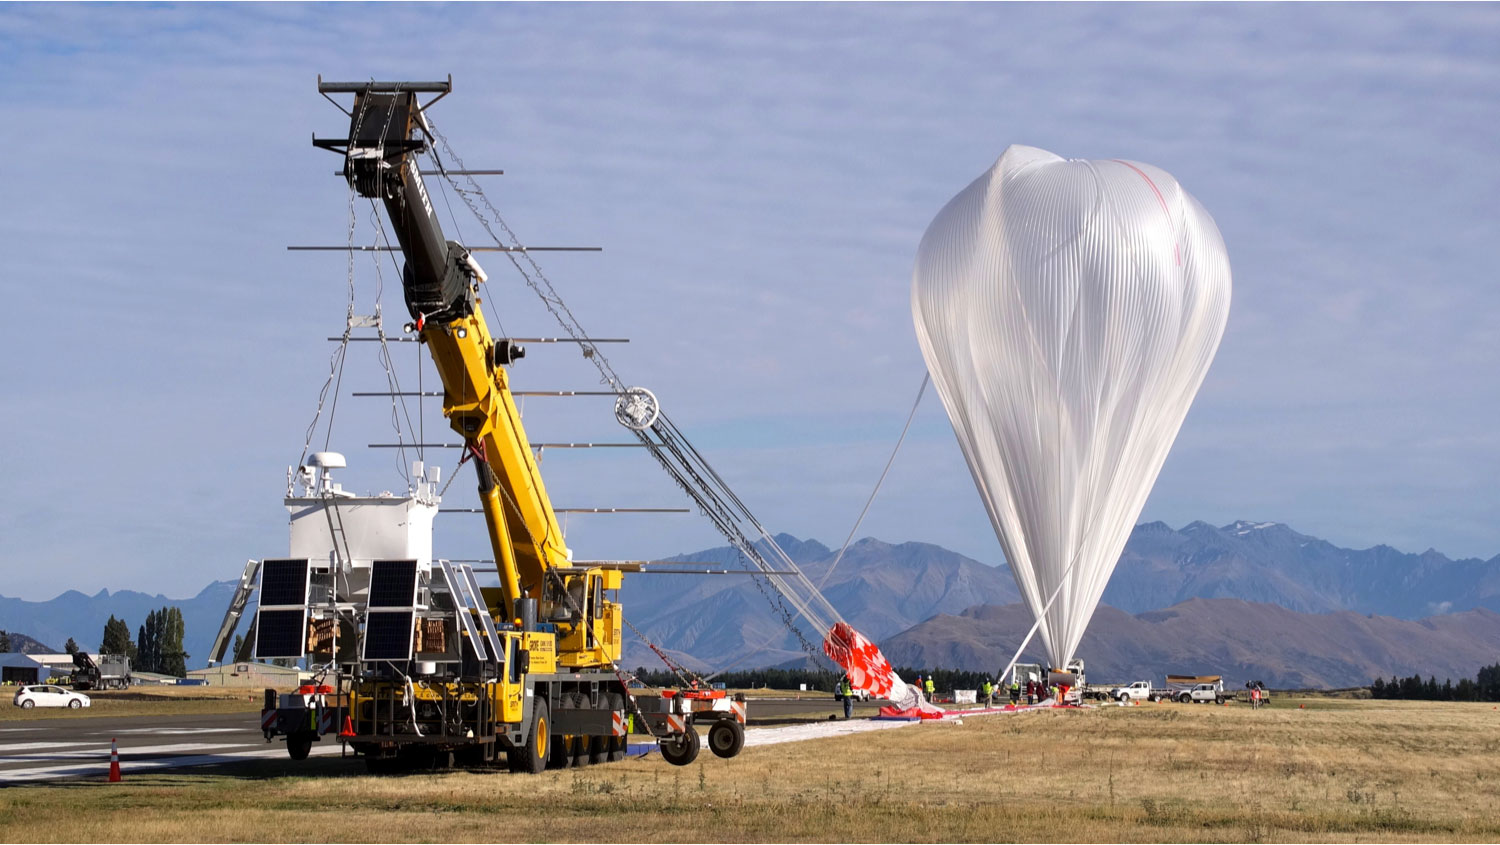
\includegraphics[width=\textwidth]{Figures/balloonLaunch.jpg} 
	\caption[Balloon launch]{Picture of a balloon launch. The payload is captured by the launch vehicle (in yellow) until the balloon is inflated and released. The parachute assembly, which is a part of the long train from the top of the payload to the bottom of the balloon, can be seen in red. Credit: NASA.}
	\label{fig:BalloonLaunch}
    \end{figure}





At float altitude, the air temperature is between \SI{230}{\kelvin} and \SI{250}{\kelvin}, while the air pressure is 0.5\% of the sea level pressure (about 5 mbar). Upper altitude winds are large-scale laminar flows that move the balloon and the payload as one. This can excite pendulum motions about the pivots underneath the balloon and at the top of the payload, which are typically of the order of a few arcminutes and have periods of a few to many tens of seconds \citep{Fixsen:1996kha}.

The payload's temperature distribution is influenced by the air temperature, infrared radiation of the Earth, and sunlight, which can result in complex temperature gradients across the instrument. A better temperature uniformity is expected for night flights, which is what BETTII is expecting.

Balloon experiments can also be affected by cosmic rays which can damage the electronics, lead to data corruption and or failures of the software/control system. However, this becomes more of an issue for long-duration balloon flights around Antarctica, during which the payloads are exposed for many weeks to the cosmic ray environment.

BETTII is expected to launch from Fort Sumner, NM, for its first engineering flight in September 2016. After a morning launch, we expect to wait until nightfall to achieve proper thermal stabilization and achieve our science goals. We expect the flight to last about \SI{16}{\hour}, although this is highly dependent on the weather and wind patterns.


\subsection{Mechanical design}

BETTII has two main structures. The first is a carbon fiber and steel truss that is used as our optical bench, and all our optical elements are attached to this structure. This was the first item that was designed in the project. The elements of this structure are built by bonding \SI{7.5}{\centi\meter} diameter hollow carbon fiber tubes to custom-made steel conical ends, that we call \textit{nose cones}. The steel nose cones are lightweight and strong, and have a threaded hole on the axis: they attach to multi-faceted steel nodes. There are three lengths of tubes on the truss. At the interface between the nose cones and the nodes, and depending on the location on the payload, we use either a combination of spherical washers and bellville washers or polypropylene washers. The difference of the washer material compensates for differential thermal contraction on the beams that form the long side of triangles.

The structure is about \SI{9}{\meter} long. It is designed to be lightweight, strong, and have a first resonant mode above \SI{20}{\hertz} to ensure fast damping of residual mechanical oscillations. We measured the first resonance peaks to be within \SI{1}{\hertz} of their expected frequency, at \SI{25}{\hertz} (see Chapter~\ref{chap:implementation}).

The entire balloon payload needs to be robust to handle 10~g vertical force and 5~g force at \SI{45}{\deg}, which are the safety guidelines from the launch facility. With an expected total mass of \SI{1000}{\kilo\gram}, we need yield strength sufficient to hold \SI{100000}{\newton} of force. 

An annotated rendering of BETTII is shown in Fig.~\ref{fig:BETTIICAD}. The gondola is what holds the truss and attaches to the balloon train. It also holds the electronics, reaction wheels, batteries, and communications to the ground. The frame is made out of 80/20 T-slotted aluminum bars that are attached together using T-inserts, and reinforced by screwed-on corner plates. The precision of this frame is of no importance to the optical alignment. 


\begin{figure}[!ht]
	\centering
	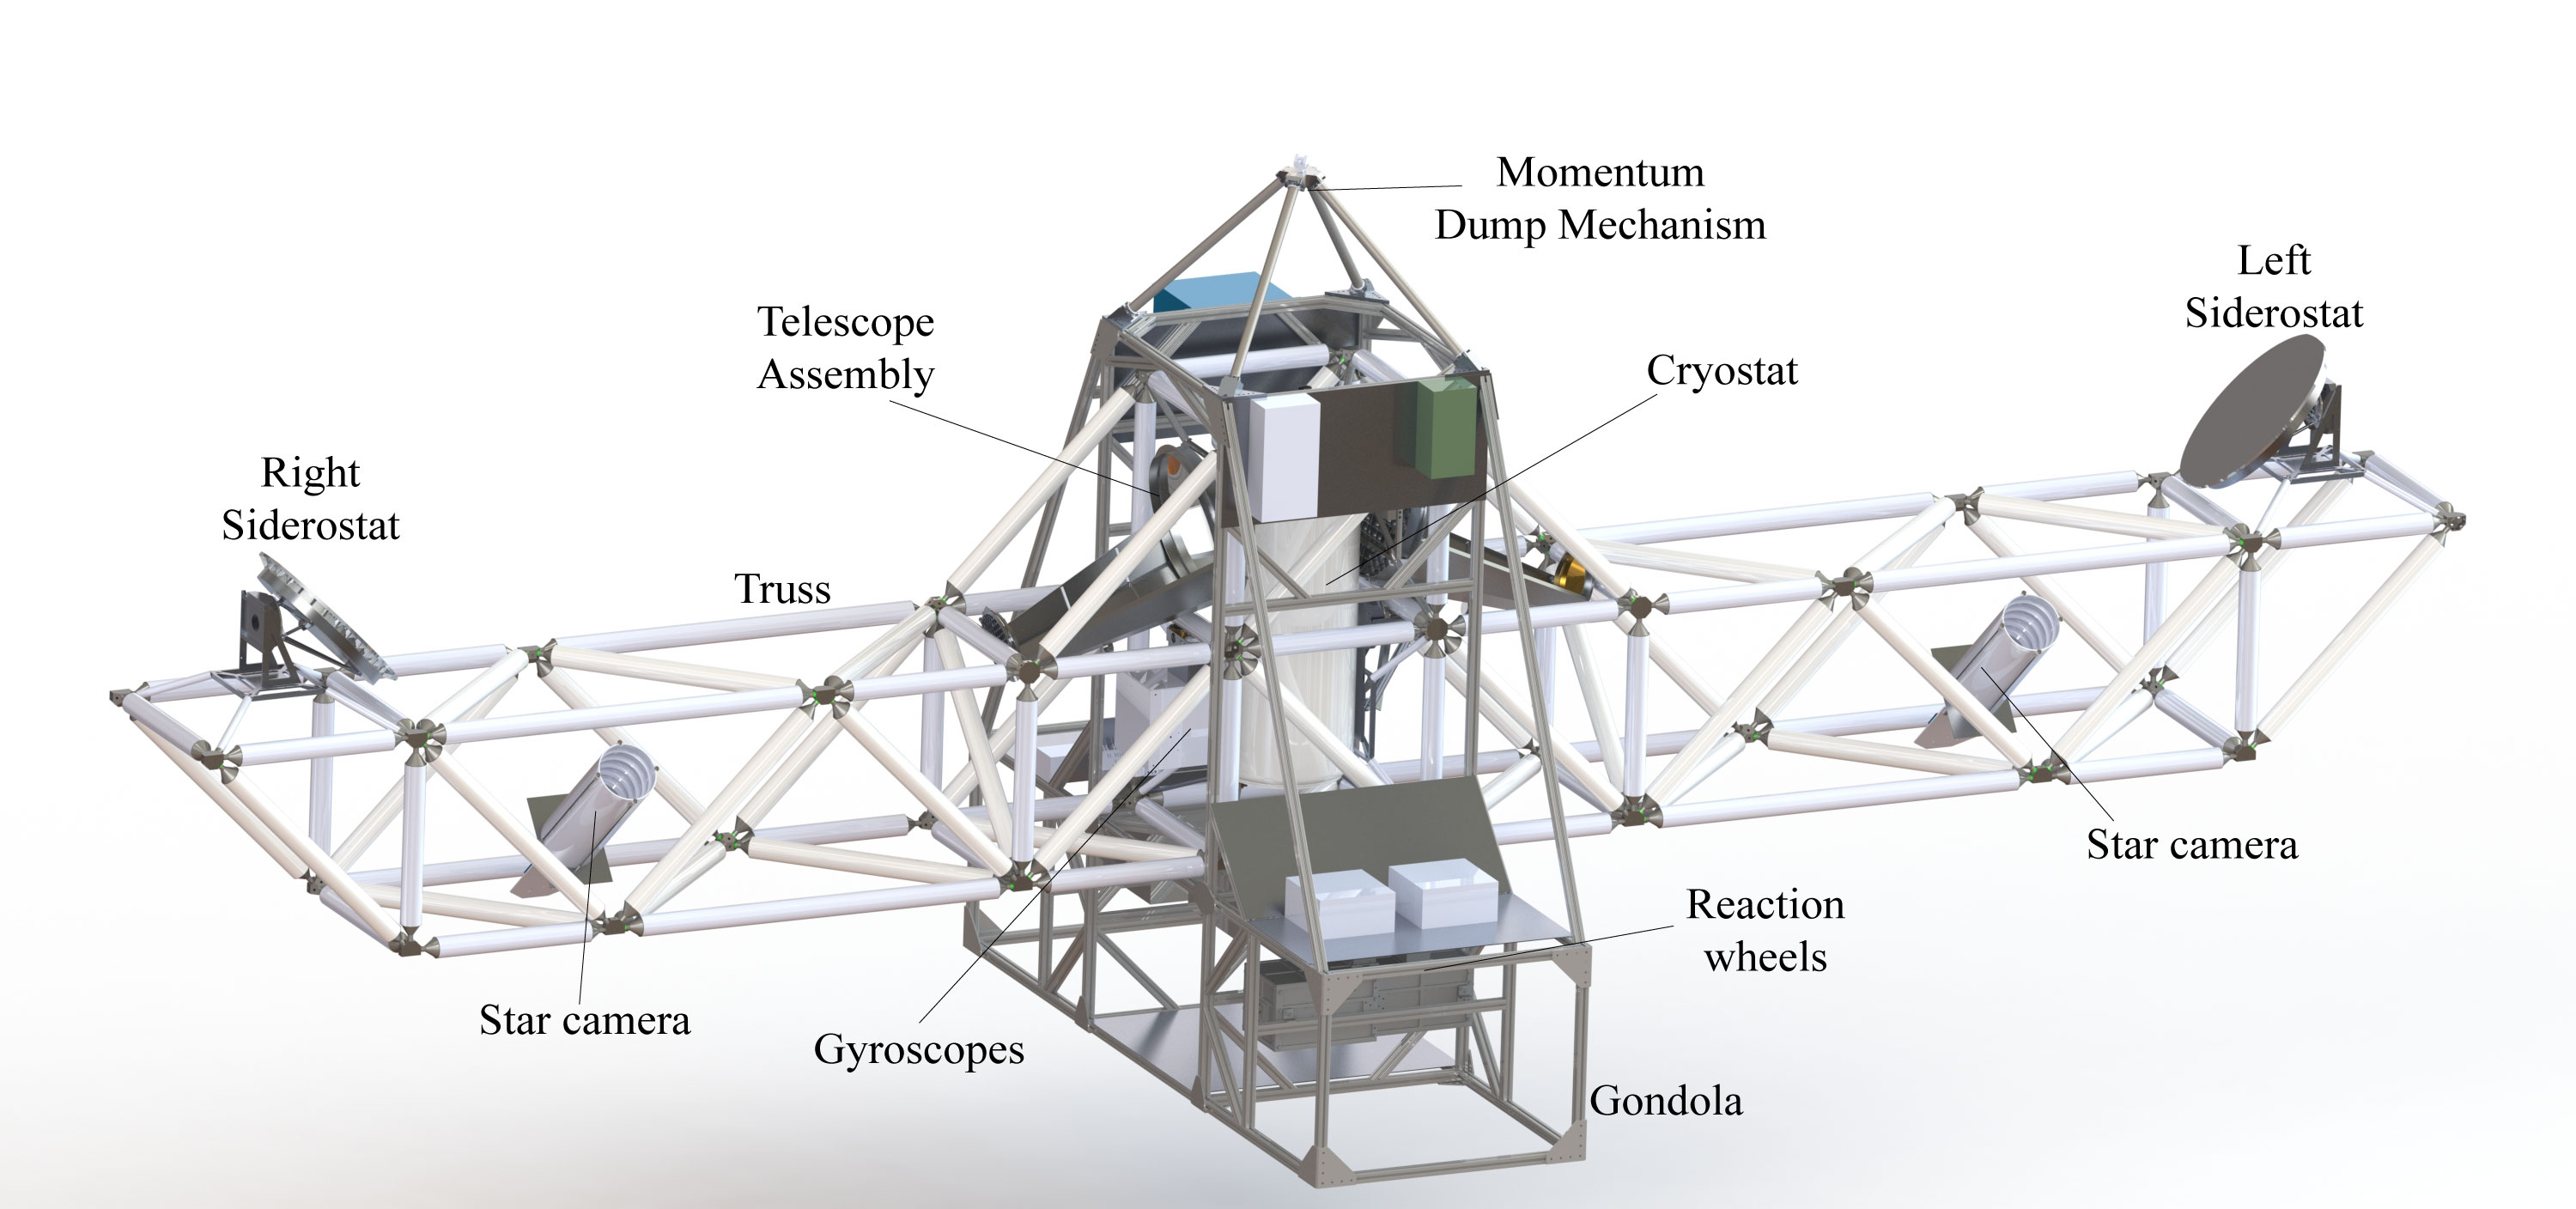
\includegraphics[width=\textwidth]{Figures/BETTII-annotated.jpg} 
	\caption[BETTII Rendering]{CAD rendering of the BETTII payload in its final state.}
	\label{fig:BETTIICAD}
    \end{figure}



The various electronic components of the system are attached to the gondola using aluminum or honeycomb aluminum plates, which are painted with white appliance paint for better thermal behavior. These plates act as radiator panels which allow us to dissipate the heat out to space.

The most critical portion of the gondola is the assembly that connects to the balloon train. This contains a single pin that needs to have the highest yield strength, since it is the only point of the payload that needs to support the entire weight. A more detailed description of the pin is presented in Section~\ref{chap:controls}.\ref{subsec:chap3momdumpmotor}.

The entire payload is designed, assembled and tested in the building 20 high bay at NASA GSFC (Fig.~\ref{fig:HighBayOpen}).
\begin{figure}[!h]
		\centering
		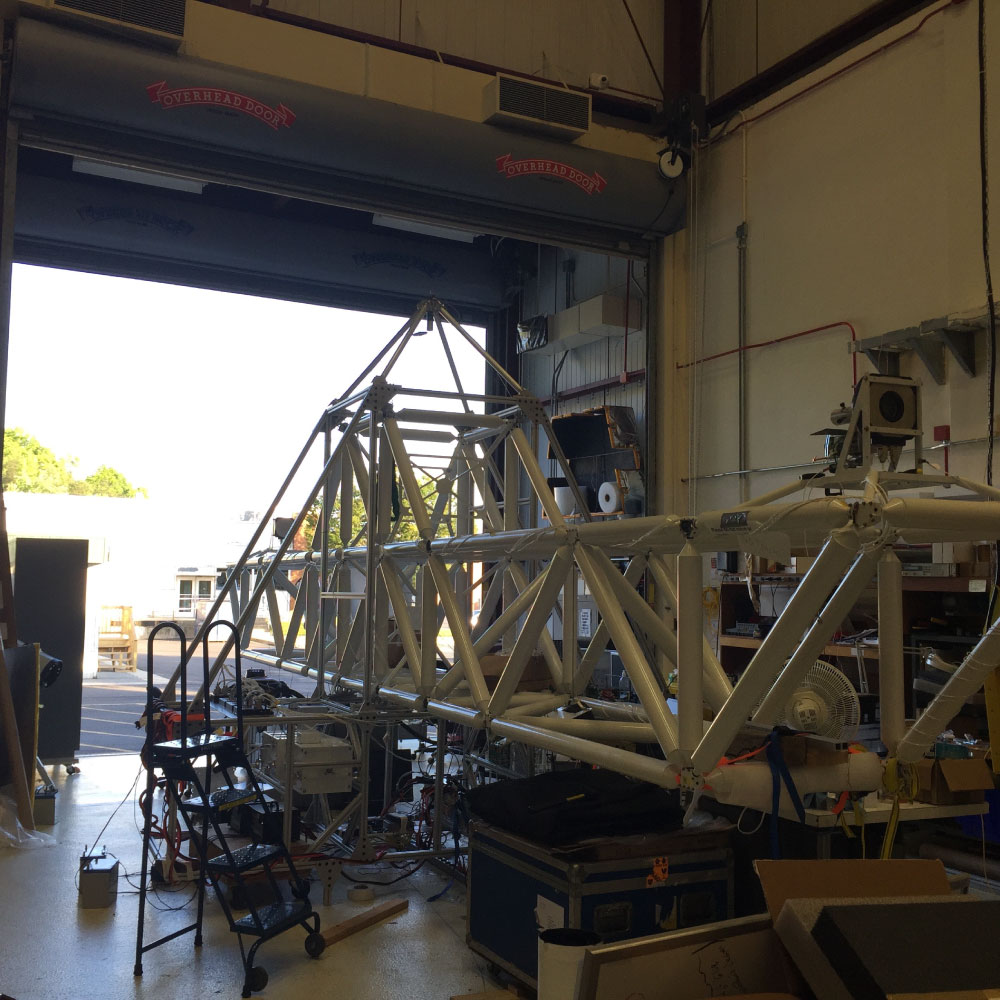
\includegraphics[width=\textwidth]{Figures/HighBayOpen.jpg} 
		\caption[Payload in high bay]{Payload in the high bay before a controls test.}
		\label{fig:HighBayOpen}
\end{figure}


\subsection{Warm optical system}

The optical system was one of the most challenging design aspects of the project. It is beyond the scope of this work to go into details about all the considerations that went into the design, but we will review some of the main aspects: the overall optics layout, and the fabrication of the telescope assemblies.

\subsubsection{Optics layout}
Because the nature of balloon payloads, there can be extensive damage to the structure during parachute opening and landing. In order to minimize the repair costs from one flight to the next, it was decided to place the telescope assemblies - which are expensive, long lead-time items - away from the edges of the truss. 

Instead, flat mirrors (that we call \textit{siderostats}) are used to redirect the light towards the telescope assemblies, which are kept close to the center of the truss where damage is expected to be minimal. 

The telescope assemblies (Fig.~\ref{fig:TelescopeAssemblyLayout}) consist of 3 powered mirrors and a folding flat. They provide a 20:1 compression ratio of the beams with reasonable tolerance on the mirror positioning. As an all-aluminum assembly, they shrink homologously as the temperature varies during the different phases of the flight, hence maintaining optical prescriptions. 

\begin{figure}[!h]
		\centering
		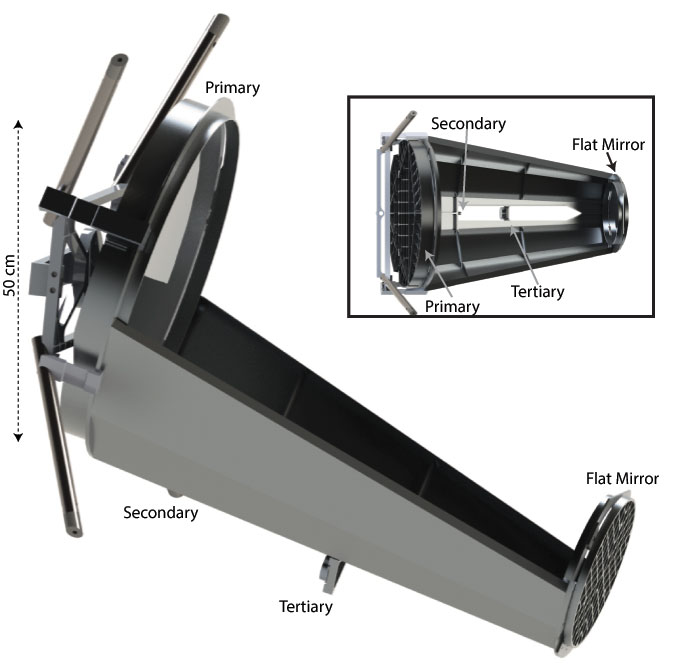
\includegraphics[width=0.7\textwidth]{Figures/TelescopeAssembly.jpg} 
		\caption[Telescope assembly layout]{Telescope assembly model and layout.}
		\label{fig:TelescopeAssemblyLayout}
\end{figure}


In order to perform double-Fourier interferometry, an extra reflection needs to be introduced in the system in order to properly combine the polarizations of the light at the beam combiner (see Fig.~\ref{fig:FTSvsDoubleFourier}). This asymmetry occurs after the telescope assemblies and before entering the cryostat. In one arm, a 3-mirror assembly (called the K-mirror assembly, or KMA) is used on a rotating stage to match the field of view rotations as the two siderostats change elevation. On the other side, a 4-mirror delay line assembly (called the Warm Delay Line, or WDL) is set at a fixed orientation. Its role is to compensate for the optical delays caused by the residual pointing errors. 

On both the KMA and the WDL (Fig.~\ref{fig:SmallAssemblies}), one of the mirrors is actuated in tip and tilt, which provides the fine control required to properly overlap the two beams at the detectors. There is an extensive discussion of the control system in Chapter~\ref{chap:controls}.

\begin{figure}[!h]
		\centering
		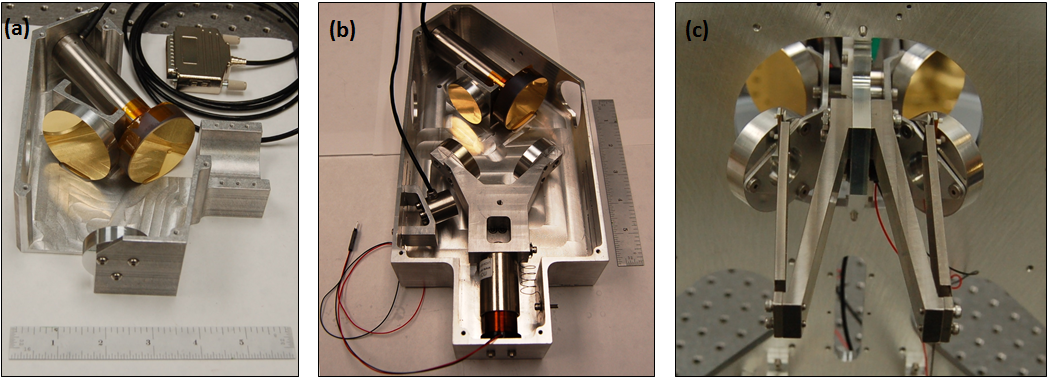
\includegraphics[width=\textwidth]{Figures/Assemblies.png} 
		\caption[Small optical assemblies]{K-Mirror Assembly, Warm Delay Line, and Cold Delay Line.}
		\label{fig:SmallAssemblies}
\end{figure}

The beams from each side enter the cryostat through thin polypropylene windows. We tested different window thicknesses and selected the \SI{15}{\micro\meter} thickness as our baseline design. %Test pieces with this window have been shown to comfortably resist about 1.5 times the atmospheric pressure, even after 50 cycles of pressurization. The maximum resistance is a little smaller when the pressurization occurs very rapidly and does not leave time to the window to deform elastically. A number of tests were done on identical batches of windows to ensure the repeatability of our test method. 
Once the beams are inside the cryostat, they are split into a NIR tracking channel, and into the FIR optics train where they are delay-modulated by the Cold Delay Line (Fig.~\ref{fig:SmallAssemblies}), combined, and image onto the detectors. A complete layout of the optics train is shown in Fig.~\ref{fig:OpticsLayout} (Dhabal \textit{et al.}, 2016, in press).


\begin{figure}[!h]
		\centering
		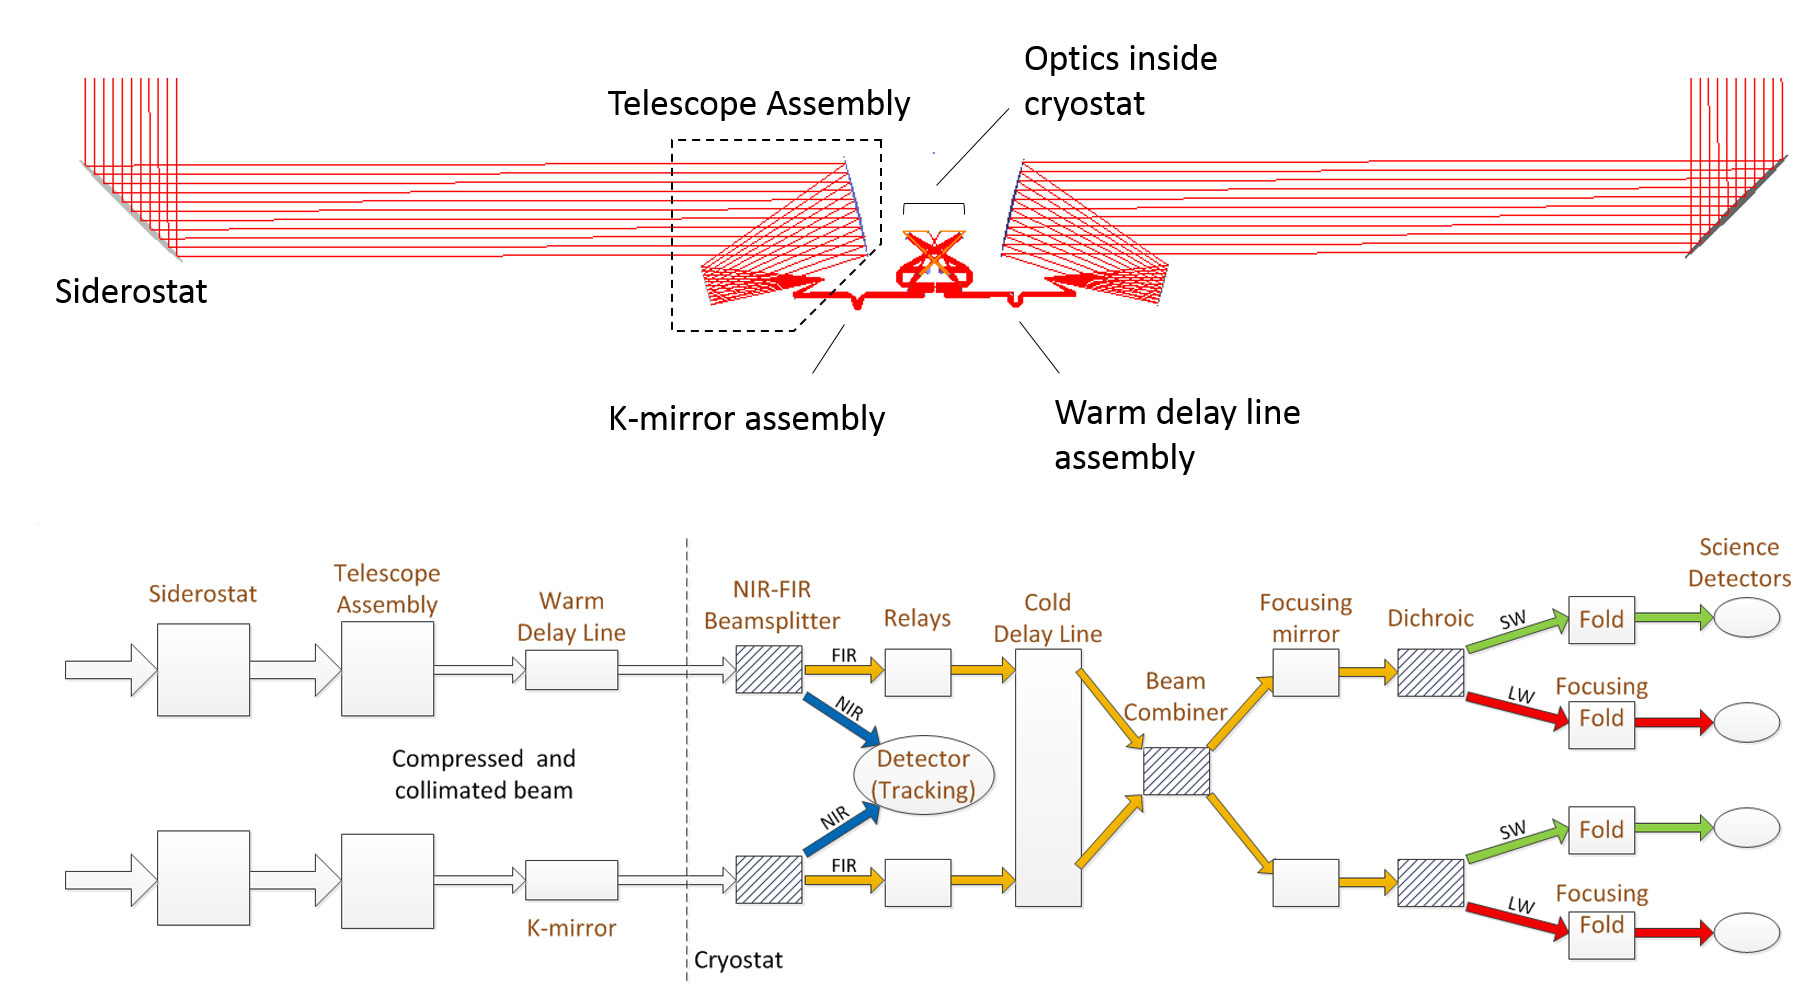
\includegraphics[width=\textwidth]{Figures/OpticsLayout.png} 
		\caption[Optics layout]{Optics layout for BETTII (Dhabal \textit{et al.}, 2016, in press).}
		\label{fig:OpticsLayout}
\end{figure}


\subsubsection{Optics manufacturing}

Despite working at relatively long wavelengths, the tolerance in the surface figure of all the mirrors is an important consideration. %Traditionally, figure errors are specified in terms of the required beam quality at the focal plane, which starts to degrade when the wavefront errors in the optical train are comparable with the wavelength of the light beam, or introduce specific aberrations. In interferometers, the fidelity of the final image is not a priority. However,
Differential wavefront errors between the two optics trains before combination will result in decreased contrast of the interferograms, which reduces our signal-to-noise ratio. As a result, the surface quality of the mirrors pre-combination needs to be much lower than a wavelength of light, since errors will stack after hitting many mirrors from both sides. We allocate \SI{2}{\um} of total wavefront error at combination, which translates to $\sim$\SI{0.23}{\um} of surface error per mirror. Given that known processes exist to manufacture small mirrors below this requirement, we relax the requirement for the primary mirrors and the siderostats to a \SI{300}{\nano\meter} r.m.s surface figure error over the entire aperture.



The company Nu-Tek, in Aberdeen, MD manufactured all of our small optics out of aluminum. The procedure includes an initial milling process, heat treatment using a method called \textit{uphill quenching}, followed by diamond turning and gold coating to avoid oxidation. 

However, very few manufacturers in the United States were able to diamond-turn the siderostats and the primary mirror assemblies, while ensuring the level of surface figure we needed. The diamond-turning process uses a slowly moving diamond blade that is controlled in 3 axes to carve out the required shape. This process requires extreme temperature stability, which is often not available in traditional machine shops. Companies which are familiar working with NASA on space missions were not affordable for a small project like us.

\begin{figure}[!h]
		\centering
		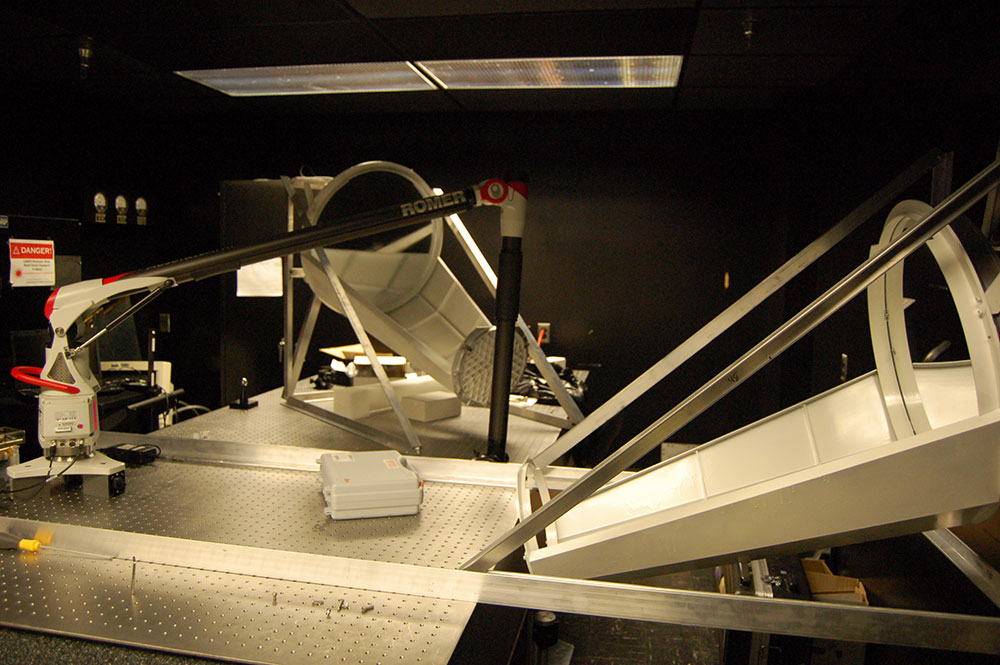
\includegraphics[width=\textwidth]{Figures/TelescopeAssemblies.jpg} 
		\caption[Telescope assemblies]{Telescope assemblies in the optics lab.}
		\label{fig:TelescopeAssemblies}
\end{figure}



The Department of Advanced Manufacturing at North Carolina State University proposed to manufacture our mirrors on a 'best effort' basis for a reasonable cost.  The results are published in Furst \textit{et al.} (2016, in press), although the surface quality has not yet been measured, due to difficulty with the equipment  and setup in the optics lab at NASA Goddard. Each telescope assembly (see Fig.~\ref{fig:TelescopeAssemblies}) has a stacked r.m.s surface figure error of \SI{300}{\nano\meter}, while the siderostats have a surface error of \SI{100}{\nano\meter} r.m.s. The siderostats are more complicated because they did not exactly fit in their diamond-turning spindle. We decided to proceed with a two-step diamond turning, where they turned two sections of the ellipse consecutively. This does not guarantee that the two areas will be at the same height since they have to unmount the mirror off the spindle. However, our models show that even if different sections of the mirrors are at different heights, the beam combination can still be successful, as the parts of the pupil that are shifted in one arm are also shifted in the other. 




\subsection{Cryogenic instrument}

The cryostat was designed by our team. Items were sent out for manufacturing to different companies and assembled in our lab. The cold volume is cooled by liquid nitrogen and helium and does not require any mechanical cryo-cooler. It is designed to operate for a duration of \SI{40}{\hour}, which should give us enough margin considering the typical lengths of balloon flights from the U.S. of about \SI{16}{\hour}. 

\begin{figure}[!h]
		\centering
		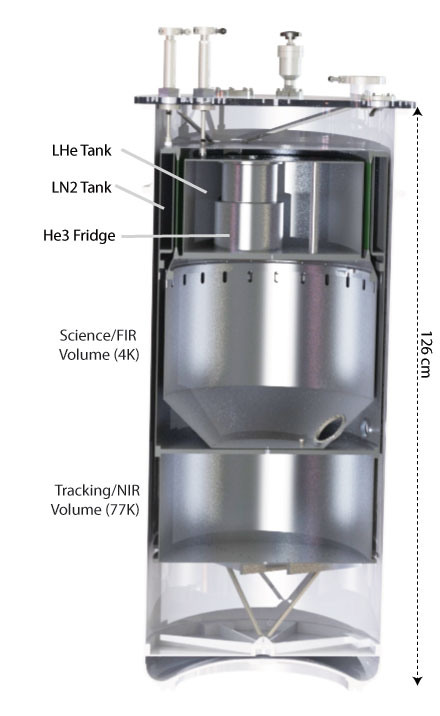
\includegraphics[width=0.6\textwidth]{Figures/Dewar.jpg} 
		\caption[Cryostat crossection]{Cryostat crossection.}
		\label{fig:CryostatCrosssection}
\end{figure}

The optics inside the cryostat are split into two sections: a near-infrared fine guidance system, and the far-infrared channels with the science detector (Fig.~\ref{fig:CryostatCrosssection}). The incoming light beam is split right after entering the cryostat with a NIR/FIR dichroic beam splitter. This custom-made filter reflects the far-IR and transmits the near-IR. At the bottom of the cryostat, in the \SI{77}{\kelvin} volume, the fine guidance sensor is composed of 12 optics and one HAWAII-1RG detector from Teledyne. 


At the top of the cryostat and attached to the \SI{4}{\kelvin} cold plate, there is a cold optics bench that holds all of the far-IR optics, filters, and the Cold Delay Line. All filters were manufactured by Cardiff University in the U.K. The layout of the optical system is shown in Fig.~\ref{fig:OpticsLayout}, and more details can be found in (Dhabal \textit{et al.}, 2016, in press). A picture of the cold optical bench with populated and aligned optics is shown in Fig.~\ref{fig:ColdBench}.

\begin{figure}[!h]
		\centering
		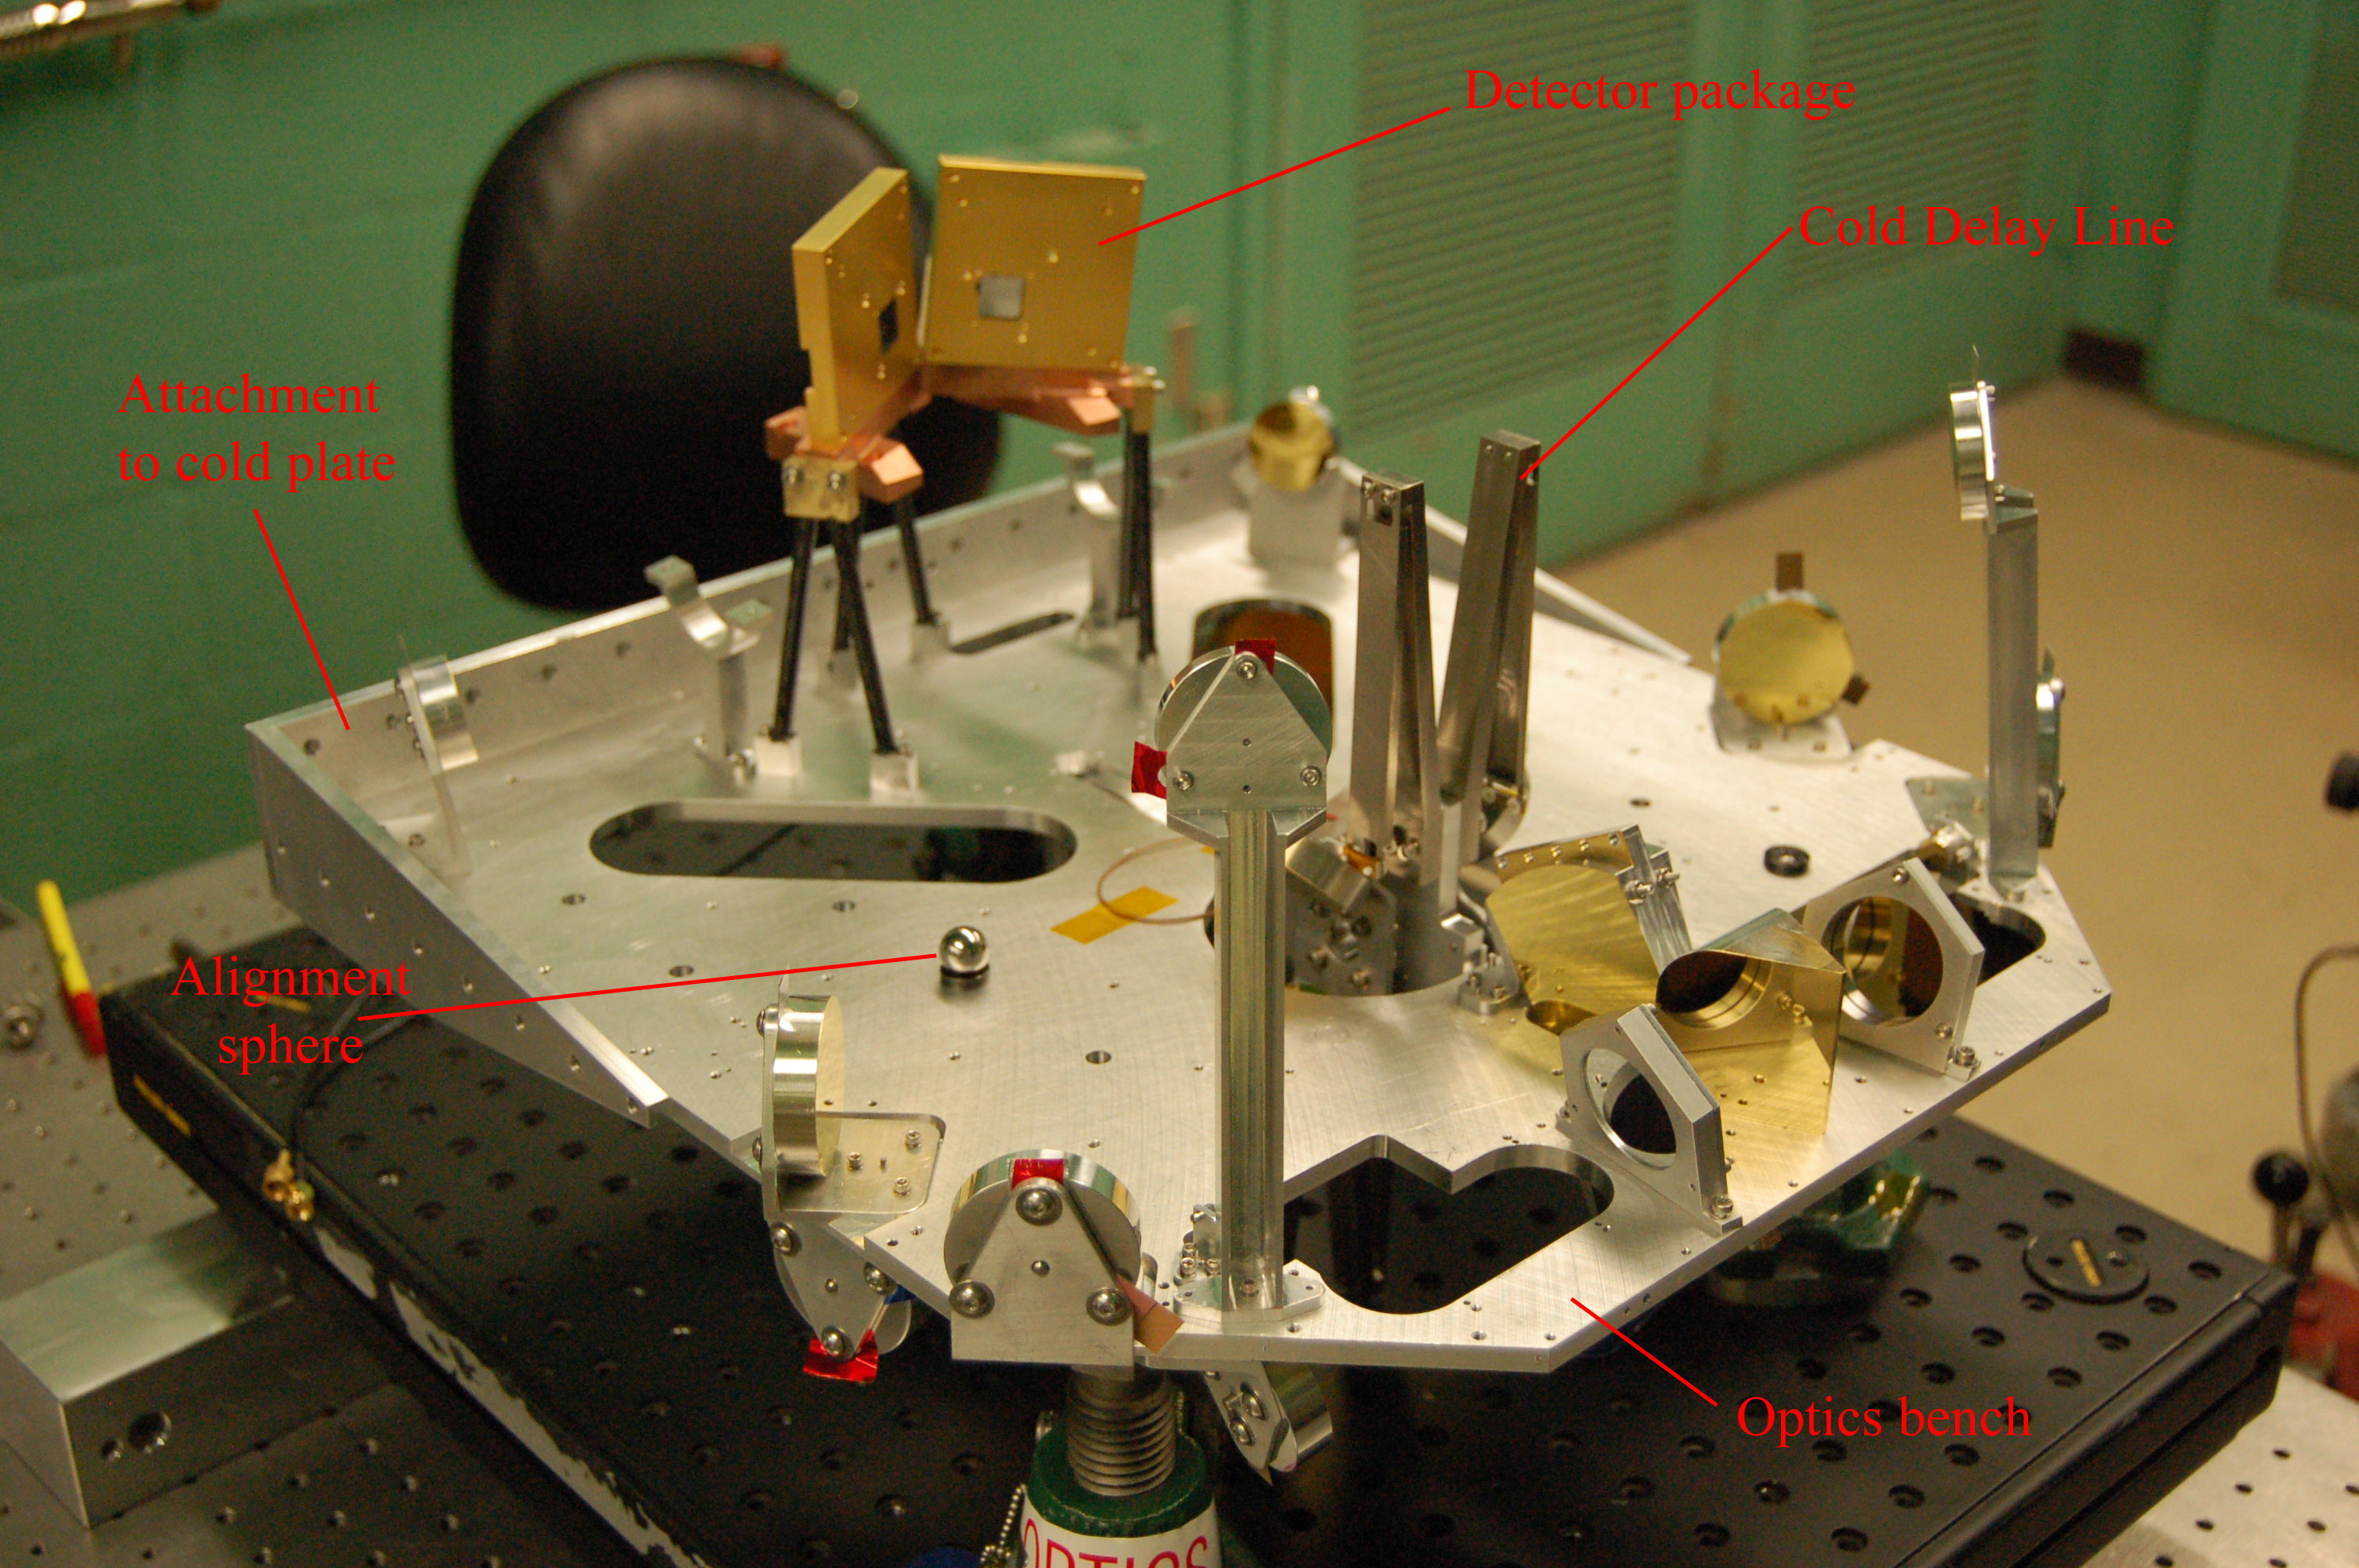
\includegraphics[width=\textwidth]{Figures/ColdBench-anottated.jpg} 
		\caption[Cold bench]{Optics on the cold bench.}
		\label{fig:ColdBench}
\end{figure}

The cold plate of the dewar is cooled down to \SI{4}{\kelvin} with liquid Helium. A ($^3$He+$^4$He) sorption refridgerator from Chase Research is used to obtain an intermediate cold finger at \SI{1}{\kelvin} and a final stage that brings down the detector temperature to $\sim$\SI{400}{\milli\kelvin}. Fig.~\ref{fig:CryostatTopPlate} shows a a picture of the top plate of the cryostat while cold. 

\begin{figure}[!h]
		\centering
		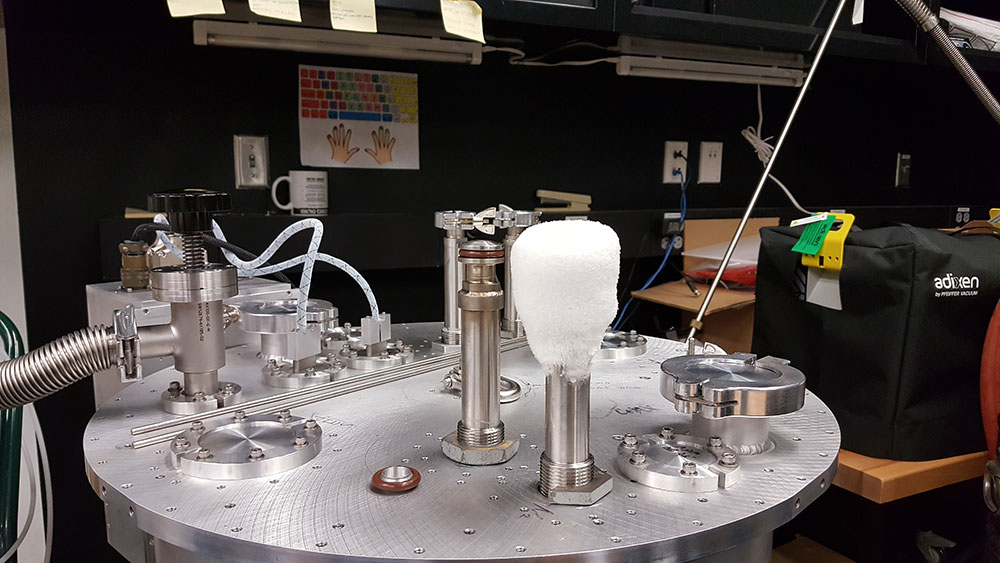
\includegraphics[width=\textwidth]{Figures/Cryostat.jpg} 
		\caption[Cryostat top plate]{Cryostat top plate during cool down.}
		\label{fig:CryostatTopPlate}
\end{figure}


At the heart of the instrument are four $9\times 9$ close-packed linear arrays of multiplexed superconducting transition edge sensor (TES) bolometers \citep{Benford:2008wk} incorporating the Backshort Under Grid (BUG) architecture \citep{Allen:2006jn}. These arrays are scaled versions of similar arrays already built for ground-based instruments \citep[e.g., GISMO,][]{Staguhn:2014jg}. Detectors are read out using advanced linear SQUID multiplexer and amplifiers. A $4\times 22$ multiplexed readout is used for each array; the extra seven channels are used for calibration signals (unilluminated pixels, “dark SQUID” channels, and an “always on” channel), allowing monitoring of all potential noise contributors \citep{deKorte:2003km}.  






\subsection{Data products \& analysis}


Once in flight the payload operations consist of pointing at a target, stabilizing the attitude motions, and scanning the delay while recording detector data. A number of operational modes are required to ensure we reach this stable observing stage, and are described in more details in Chapter~\ref{chap:controls}. 

Individual scans will last for a nominal duration of \SI{2.5}{\second}, and consist of \si{1024} individual detector frames, which are matched to a given \OPD. To increase the signal-to-noise ratio (\SNR), we expect to stack \SI{10}{\minute} worth of data, which corresponds to 200 scans. For this duration, we expect that the change in the baseline angle due to the rotation of the Earth is negligible. It is critical to correctly stack the interferograms, as \OPD errors from scan to scan can significantly reduce the fringe contrast (see Chap.~\ref{chap:phasenoisepaper}).

To describe post-processing, let's consider a \SI{10}{\minute} cube which is the {\OPD}-corrected stack of images from the 200 individual scans. The cube has a crossection of $9\times 9$ (which is the size of an individual detector frame), and a depth of 1024 frames. For each frame, the intensity of each source in the detector is determined for each \OPD, and combined into interferograms. We repeat the process for the same field observed at different baseline angles. 

Using starting points involving our existing SOFIA multi-wavelength observations, as well as the IRAC images, these interferograms will help determine the multiplicity of bright sources, their individual SED, and their position relative to the large-scale extended emission. 

If BETTII had more baseline lengths and the reconstructed cubes filled the aperture more densely, it would be possible to feed them directly to an inversion software that was developed in Dr. Juanola-Parramon's Ph.D. thesis \citep{Juanola:2016}, which provides a final datacube corresponding to the images as a function of wavelength, with the spectral resolution that the user chooses. 

\begin{figure}[!h]
	\centering
	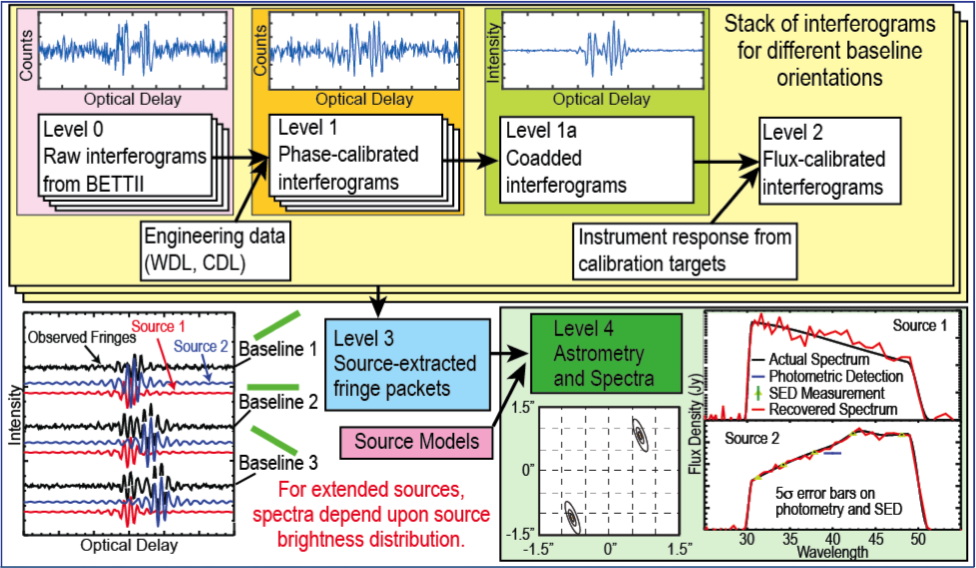
\includegraphics[width=\textwidth]{Figures/DataProcessing.png}
	\caption[Data processing]{BETTII data processing steps.}
	\label{fig:dataProcessing}
    \end{figure}



\newpage
\section{Sensitivity analysis}

Early in my involvement with BETTII, I led the effort in trying to estimate the sensitivity of our instrument, in order to select relevant scientific targets, but also find astronomical calibrator objects which would help us understand the systematics of our payload.

This section summarizes the findings and gives details on the methods and equations we used. We were able to derive a new formalism to estimate the spectral sensitivity of double-Fourier interferometers for point sources. Our method uses propagation of gaussian errors through Fourier transforms, and is described in detail in Chapter~\ref{chap:phasenoisepaper}. This can be useful to determine the sensitivity of other types of instruments, such as a space-based follow-up of BETTII, which we briefly discuss in the conclusion of this work.

\subsection{Instrument and observing parameters}

\renewcommand{\arraystretch}{1.5}
\begin{table}
\small
\caption[Instrument parameters]{Instrument design parameters for BETTII.}
\vspace{-0.5cm}
\label{tab:instrumentParameters}
\begin{longtable}{P{5cm}|c|c|P{1.5cm}|P{3cm}}
\toprule													
Parameter	&	\multicolumn{2}{c|}{          		 Value		} 			&	Units	&	Science driver/impact	\\
\midrule													
\multicolumn{5}{c}{		Top-level parameters	}										\\
\midrule
Input aperture	&	\multicolumn{2}{c|}{		0.196		}			&	\si{\raiseto{2}\meter}	&	Sensitivity	\\
Baseline length	&	\multicolumn{2}{c|}{		8		}			&	\si{\meter}	&	Angular resolution	\\
Detector pixels	&	\multicolumn{2}{c|}{	$	9\times 9	$	}			&	pixels	&	Wide FOV\\
Detector quantum efficiency	&	\multicolumn{2}{c|}{		70	\%	}			&		&	Sensitivity	\\
Integration time per full frame	&	\multicolumn{2}{c|}{		2.5		}			&	\si{\milli\second}	&	Sensitivity	\\
Time per baseline orientation	&	\multicolumn{2}{c|}{		10		}			&	\si{\minute}	&	Sensitivity	\\
Number of data points per scan	&	\multicolumn{2}{c|}{		1024		}			&	points	&	Wide FOV	\\
OPD range required	&	\multicolumn{2}{c|}{		8.2		}			&	\si{\milli\meter}	&	Wide FOV \& spectral resolution	\\
\midrule													
\multicolumn{5}{c}{		Optical system	}										\\
\midrule													
	&		Band 1		&		Band 2		&		&		\\
Central wavelength	&		40		&		82		&	\si{\micro\meter}	&	Study YSOs	\\
Fractional bandwidth	&		62.5	\%	&		54.9	\%	&		&	SNR at ZPD	\\
Field of view	&		2		&		3		&	\si{\arcmin}	&	YSO regions	\\
Etendue per pixel	&	\num{	8.2E-10	}	&	\num{	1.8E-09	}	&	\si{\raiseto{2}\meter\steradian}	&	Sensitivity	\\
Estimated efficiency	&		20	\%	&		24	\%	&		&	Sensitivity	\\
Pixel angular size	&		13.32		&		19.72		&	\si{\arcsec}	&	Wide FOV	\\
Primary full width half max	&		17.31		&		35.49		&	\si{\arcsec}	&	Sensitivity	\\
\bottomrule																					
\end{longtable}
\caption*{\textbf{Notes}: Instrument parameters that flow from the science requirement of \ang{;;0.5} and \ang{;;1} spatial resolution in bands 1 and 2 respectively, and spectral resolution $\R = 10$ in both bands.}
\end{table}


Table~\ref{tab:instrumentParameters} represents the key instrument parameters that are relevant for the sensitivity estimation of the two science channels of BETTII. The main impact of each parameter on some aspects of the science is shown. A detailed, custom calculator tool that we developed compiles most of the instrument parameters that flow down from these requirements, which in turn serve as design baseline for various subsystems. For example, the "OPD range required" is a derived output, depending on the baseline length, the field of view and the required spectral resolution.


\subsection{Far-IR background noise estimation}



We proceed to an estimation of the known far-IR background noise contributions from sources in thermal equilibrium. We assume that each source of noise emits like a Planck function \Bnu with a certain emissivity $\epsilon$. In Table~\ref{tab:noiseparams}, we list the number of photons generated per second for the amount of solid angle seen by a single pixel (with the exception of the atmospheric contribution, which is treated separately). The thermal emission is weighted by the normalized transmission function, which was measured in the laboratory (Fig~\ref{fig:BETTIITransmission}). By far the strongest contributors from our system are the warm optics and the cryostat's polypropylene window.
 

In addition to the noise of our own system and the astronomical background, we need to take into account the noise generated by the atmosphere, which results in a more complex calculation. For best accuracy, we use quantities from \cite{Harries:1980cva}, who measured the actual sky radiance in a large range of wavelengths from balloon altitudes. We obtain a radiance of \SI{0.16}{\watt\per\raiseto{2}\meter\per\steradian} and \SI{0.07}{\watt\per\raiseto{2}\meter\per\steradian} for band 1 and 2 respectively. This corresponds to \num{2.6e10}~photons~\si{\per\second} and \num{5.2e10}~photons~\si{\per\second}, respectively. 

\renewcommand{\arraystretch}{1.5}
\begin{table}
\small
\caption{Thermal noise contributors}
\label{tab:noiseparams}
\vspace{-0.5cm}
\begin{longtable}{P{2.5cm}ccP{2cm}P{2cm}p{3cm}}
\toprule
Noise source	&		T (K)		&		Emissivity		&		Photons~\si{\per\second} Band 1		&		Photons~\si{\per\second} Band 2		&	Reference	 \\
\midrule
Warm optics	&	\num{	240	}	&	\num{	0.1	}	&	\num{	1.38E+11	}	&	\num{	9.97E+10	}	&	Assumes 99\% per mirror	\\
Window	&	\num{	240	}	&	\num{	0.02	}	&	\num{	2.76E+10	}	&	\num{	1.99E+10	}	&	Lab measurements	\\
Zodi dust	&	\num{	245	}	&	\num{	3.00E-07	}	&	\num{	2.92E+05	}	&	\num{	3.41E+05	}	&	\cite{Fixsen:2002da}	\\
Galactic Cirrus	&	\num{	20	}	&	\num{	1.23E-04	}	&	\num{	1.79E+01	}	&	\num{	7.67E+04	}	&	\cite{Bracco:2011gw}	\\
Zodi scattering	&	\num{	5800	}	&	\num{	1.00E-13	}	&	\num{	1.47E+01	}	&	\num{	1.31E+01	}	&	\cite{Fixsen:2002da}	\\
CIB	&	\num{	18.5	}	&	\num{	1.30E-05	}	&	\num{	2.19E+00	}	&	\num{	9.68E+03	}	&	\cite{Fixsen:1998br}	\\
Instrument	&	\num{	4	}	&	\num{	1	}	&	\num{	8.3E-27	}	&	\num{	3.60E-07	}	&	Conservative estimate	\\
CMB	&	\num{	2.728	}	&	\num{	1	}	&	\num{	1.02E-45	}	&	\num{	9.35E-17	}	&	\cite{Fixsen:1996di}	\\
\bottomrule
\end{longtable}
\caption*{\textbf{Notes}: The calculator was designed to be scalable to designing a space mission, which is why we kept track of terms which are negligible compared to the main contributors. In space, the warm optics and window contributions would be significantly reduced and more comparable to the other terms. These quantities do not yet include the losses from the instrument's throughput}
\end{table}

\begin{figure}[!h]
	\centering
	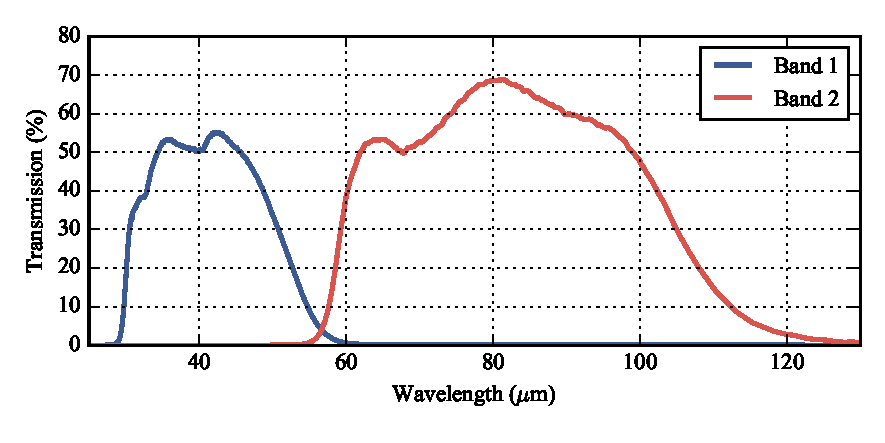
\includegraphics[width=\textwidth]{Figures/BETTII_transmission.pdf}
	\vspace{-0.5cm}
	\caption[BETTII Transmission curves]{BETTII total transmission curves $\Tbp(\lambda)$ from all cold filters, excluding the beam combiner, cryostat window, and NIR/FIR dichroic. Bands are shown in different colors.}
	\label{fig:BETTIITransmission}
    \end{figure}



To know how much power is actually reaching the detectors, we need a measurement of our optical throughput. The throughput is the product of the efficiencies of the various elements along the optical train: the mirrors, the cryostat window, the NIR/FIR dichroic, and all the cold filters. The latter multiply to give the transmission profile shown in Fig.~\ref{fig:BETTIITransmission}, which we call $\Tbp$. We write $f_\textrm{arm1->detN}$ (resp. $f_\textrm{arm2->detN}$) the throughput of light from arm M (resp. arm 2) falling on the detector N, where N = {1, 2}:
\begin{align}
f_\textrm{arm{1,2}->det{1,2}}(\lambda) &= \tau_\textrm{combiner}\tau_\textrm{window}\tau_\textrm{dichroic}r^{N_\textrm{mirrors}}\Tbp(\lambda) \\
& \approx 0.38\times \Tbp(\lambda),
\end{align}
where we have used lab measurements to estimate $\tau_\textrm{window}\approx 0.98$, $\tau_\textrm{dichroic}\approx 0.95$, $\tau_\textrm{combiner}\approx 0.5$ and $r\approx 0.99 $ is the far-IR reflection of each warm mirror, in both bands. There are $N_\textrm{mirrors} = 9$ within the warm optics train on the left side, and 8 on the right side. Until we obtain precise measurement of the throughput of each element as a function of wavelength, we consider that this extra factor is wavelength-independent and represents an average over the band. This is valid since most of these materials do not have steep dependence at such a long wavelength. The transmission $\Tbp(\lambda)$ has an average of 27\% (resp. 31\%) for band 1 (resp. 2) respectively, so the throughput amounts to about $\sim 10\%$ (resp. $\sim 12\%$) efficiency for the light coming from one arm falling onto one detector. 

\renewcommand{\arraystretch}{1.5}
\begin{table}
\small
\caption[Power and NEP contributors]{Estimated power and NEP contributors for a single detector pixel.}
\vspace{-0.5cm}
\begin{longtable}{P{3cm}|P{2cm}|P{2cm}|P{2cm}|P{2cm}}
\toprule																	
Noise source	 &		\multicolumn{2}{c}{		Power reaching the detector (pW)			}	 &		\multicolumn{2}{c}{		NEP (\SI{e-16}{\watt\per\raiseto{0.5}\hertz})			}	\\
	&		Band 1		&		Band2		&		Band 1		&		Band2		\\
\midrule																	
Warm optics	 &	\num{	92	}	&	\num{	45	}	 &	\num{	9.6	}	&	\num{	6.7	}	\\
Atmosphere	 &	\num{	18	}	&	\num{	24	}	 &	\num{	4.6	}	&	\num{	4.9	}	\\
Window	 &	\num{	21	}	&	\num{	9	}	 &	\num{	4.3	}	&	\num{	3.0	}	\\
Detectors	 &		-		&				 &	\num{	5	}	&	\num{	5	}	\\
\midrule																	
Total	&		131		&		77		&		17		&		10		\\
\bottomrule																						\end{longtable}
\caption*{\textbf{Notes}: These values are lower than the ones cites in \citet{Rinehart:2014gk} and \citet{Rizzo:2015gf} since we now have more precise measurements of the transmission as a function of wavelength.}
\label{tab:powerNEP}
\end{table}


After accounting for all losses, we approximate the total noise power per pixel as:

\begin{equation}
P_\textrm{pix} = (f_\textrm{arm1->detN}+ f_\textrm{arm2->detN})N_\textrm{Photons~\si{\per\second}}E_\textrm{ph}\QE,
\end{equation}
where $N_\textrm{Photons~\si{\per\second}}$ is the total number of photons per second per pixel from the warm optics, the window, and the atmosphere, which are the three main contributors of noise (see Table~\ref{tab:noiseparams}). We also use the photon energy $E_\textrm{ph}$ and detector efficiency of the detector, $\QE\approx 0.7$. Throughout most the design phase of BETTII, this equation was used for the band-averaged quantities, for lack of better knowledge of the exact wavelength dependence of the various optical components. However, this is also valid on a finer scale and can be integrated over wavelength to provide more accurate estimates. In Table~\ref{tab:powerNEP}, we used our knowledge of the bandpass transmission and integrate over the band. The Noise Equivalent Power (NEP), a common measure of noise in the far-IR, is calculated as $\NEP = \sqrt{2P_\textrm{pix}E_\textrm{ph}}$. Note that the detectors are designed to contribute less than 30\% of the total estimated photon NEP, so that their noise contribution is negligible.


\subsection{Interferometric visibility budget}

Estimating the noise from each arm separately can help us determine important quantities such as the photon loading and NEP, which can be used to design the detectors. However, the scientific signal from an interferometer also depends on how well the two arms combine. This is roughly a measure of how symmetric the optical system is. In table~\ref{tab:visbudget}, we identify two kinds of error contributions: the static contributors, which are caused by differential wavefront errors (WFE), amplitude mismatch, polarization errors and pupil area overlap. These are caused mostly by misalignments of the optics along each train, or by errors in the manufacturing of the mirror surfaces. Second, we have the dynamic contributors, which are caused by \OPD errors and differential tip/tilt. These are errors which need to hold over the timescale corresponding to a single data point, so about \SI{2.5}{\milli\second}. The OPD errors correspond to fast uncorrected motion of the delay lines, while the differential tip/tilt corresponds to an error is co-aligning the two beams at the detector. Note that in Chap.~\ref{chap:phasenoisepaper}, we discuss the various timescales involved with the \OPD motions. In this table and for the calculation of the visibility, we only take into account the instantaneous, un-recoverable error in \OPD. The error in \OPD over longer timescales, resulting in a decrease in \SNR as we co-add consecutive interferograms, is not taken into account here. For reference, the equations are explicitly stated here, as we have found it handy to gather them all in one single place. The derivation for most equations can be found in \citet{Lawson:2000vf}.

\renewcommand{\arraystretch}{1.5}
\begin{table}[!h]
\small
\caption[Interferometric visiblity budget]{Interferometric visiblity budget.}
\label{tab:visbudget}
\begin{longtable}{P{3cm}|P{1cm}|P{1cm}|P{4cm}|P{1.5cm}|P{1.5cm}}
\toprule													
Term	& 	Symbol	& 		Alloc.		& 	Effect on visibility	& 	\multicolumn{2}{c}{\Vloss}			\\
	&		&				&		&	Band 1	&	Band 2	\\
\midrule													
\multicolumn{6}{c}{Static contributors}													\\
\midrule													
Total WFE in mirror surfaces	& 	\sigWFE	& 	\SI{	2	}{\micro\meter}	& 	$\exp(-[2\pi\sigWFE/\lambda]^2)$	& 	0.906	& 	0.977	\\
Amplitude mismatch	& 	$R$	& 		95	\%	& 	$2/(R^{1/2}+R^{-1/2})$	& 	0.999	& 	0.999	\\
Polarization effects	& 	$\theta$	& 	\SI{	12	}{\degree}	& 	$\cos(\pi\theta/180/2)$	& 	0.995	& 	0.995	\\
Pupil area overlap	& 	\foverlap	& 		90	\%	& 	\foverlap	& 	0.900	& 	0.900	\\
\midrule													
\multicolumn{6}{c}{Dynamic contributors}													\\
\midrule													
Error in OPD knowledge	& 	\sigOPD	& 	\SI{	2	}{\micro\meter}	& 	$\exp(-[2\pi\sigOPD/\lambda]^2)$	& 	0.906	& 	0.977	\\
Differential tip/tilt	& 	\sigtt	& 	\ang{;;	1.5	}	& 	$2J_1(\pi D\sigtt/\lambda)/(\pi D\sigtt/\lambda)$	& 	0.990	& 	0.998	\\
\midrule													
\multicolumn{3}{r}{Total visibility}							&	$\Pi(\Vloss)$	&	0.726	&	0.851	\\
\bottomrule											
\caption*{\textbf{Notes}: The dynamic contributors need to hold true for \SI{2.5}{\milli\second}, and consist of the residual amount that cannot be corrected in post-processing.}
\end{longtable}
\end{table}

\subsection{Science channel estimated sensitivity}

Now that we know the noise per pixel and the efficiency of the interferometric beam combination, we can determine the \SNR for a single source of known flux. For this, we use the formalism by \citet{Mighell:2005fwa} who derive the proper equation for a matched filter representing a point-spread function (PSF) discretized on a noisy detector array. The efficiency $\etamf$ of the matched filter is the inverse of the square root of the effective background area of the PSF, $\beta = 4\pi \mathcal{S}^2$, where $\mathcal{S}$ is the standard deviation of the PSF in pixels, $\mathcal{S} = \frac{0.42\lambda/D}{\theta_\textrm{pix}}$. We obtain $\etamf \approx 0.55$ and $0.39$ for band 1 and 2 respectively.

This matched filter efficiency is due to the uneven spread of the light from a PSF onto multiple pixels, and corresponds to the error in fitting the detector to the PSF assuming an even noise floor among all pixels. Pixels with more photons will have more \SNR, hence should be weighted more when attempting to extract the flux from the PSF. In this sense, using a matched filter is a best-case scenario. Another approach would consist of simply dividing the PSF area by the area of one single pixel, which is a worst-case alternative that would lead to efficiencies of 0.13 and 0.07 in band 1 and band 2 respectively. In what follows, we are using the optimistic approach and assume we can recover the flux from the PSF using matched filtering. 

We define the Minimum Detectable Line Flux (\MDLF) as the flux per pixel which corresponds to a $\SNR = 1$:
\begin{align}
\MDLF = \frac{\NEP}{(f_\textrm{arm1->detN}+ f_\textrm{arm2->detN})\Area\sqrt{2\Tint}},
\end{align}
where $\Tint = \SI{2.5}{\milli\second}$ corresponds to the integration time per pixel (or detector frame). The \MDLF is expressed in \si{\watt\per\raiseto{2}\meter}.

The Minimum Detectable Flux Density (\MDFD) is the \MDLF divided by the bandwidth. This is expressed in \si{\watt\per\raiseto{2}\meter\per\hertz} and can be converted to \si{\jansky}.

The faintest detectable interferometric point source with $\SNR = 1$ is then given by $\Smin= \MDFD/\Vi/\etamf$, where the \MDFD is increased due to the interferometric visibility losses and the spreading of the photons onto multiple pixels of the detector. \Smin represents the smallest flux density that leads to an $\SNR = 1$ within a single scan.

Co-adding consecutive scans will improve the \SNR considerably, but it will also introduces errors and inefficiencies. We quickly realized the impact of systematic errors in co-adding scans, so a significant amount of effort went into understanding the behavior of the various error contributions, and analyzing mitigation strategies. The result of this investigation was published in \citet{Rizzo:2015gf}, and is shown here in Chap.~\ref{chap:phasenoisepaper}. In that chapter, we discuss the meaning and importance of the phase noise or \OPD noise, and quantify the impact on the sensitivity. The \OPD noise arises when residual uncertainties in the knowledge and control of the \OPD result in errors while co-aligning and co-adding consecutive interferograms. For the rest of this discussion, we will assume that the \OPD noise amounts to \SI{5}{\micro\meter} r.m.s over 200 consecutive scans.

Using the formulas derived in Chap.~\ref{chap:phasenoisepaper}, we can now correctly determine the \SNR in the co-added interferograms. However, co-added interferograms are not the only goal of BETTII. Although interferograms allow for the distinction between multiple, nearby point sources, most of the scientific information is retrieved by analyzing the spectrum of each source in the field by taking the Fourier transform of the interferogram. Hence, we want to characterize the spectral sensitivity of the instrument, and establish this metric as the default observing metric for our science.

A summary of the results is presented in Table~\ref{tab:BETTIIsensitivity}.

\begin{table}[ht!]
\begin{center}
\caption{BETTII sensitivity estimates}
\label{tab:BETTIIsensitivity}
\vspace{-0.5cm}
\begin{longtable}{cccc}
\toprule
  Quantity   & Band 1 &  Band 2 & SNR Target \\
     \midrule 
 \multicolumn{4}{c}{\textbf{Single scan (\SI{3}{\second})}} \\
MDFD & 77 Jy  & 113 Jy & $\SNR_\mI = 1$\\ 
\midrule
\multicolumn{4}{c}{\textbf{Normal observing (200 scans, 10 min)}} \\
MDFD & 5 Jy  & 8 Jy & $\SNR_\mI = 1$\\ 
\bottomrule 
\end{longtable} 
\caption*{\textbf{Notes}: $\SNR_\mI$ represents the \SNR in the interferogram.}
\end{center}
\end{table} 


\subsection{Tracking channel estimated sensitivity}
A similar sensitivity analysis is done for the tracking channel. This is simplified somewhat since the tracking channels consists only of two cameras, and does not involve beam combination. The levels of background noise are less obvious to estimate. We primarily use the findings of \citet{Matsumoto:1994io}, which measured \SI{2}{\micro\meter} emission line strengths from balloon altitude. This emission is thought to arise from a thin layer of OH radicals at $\sim\SI{100}{\kilo\meter}$ altitude, and is sometimes referred to as \textit{airglow}. Using the measurements by these authors, who span multiple balloon flights in the 60s and 70s, we obtain an average radiance in the NIR bands of $\Rnir~\approx~\SI{1e-4}{\watt\per\raiseto{2}\meter\per\steradian}$. According to our estimates, this is two orders of magnitudes lower than the brightest astronomical noise source in the NIR, which is the zodi scattering.

Balloon altitudes provide significantly better atmosphere transmission in the NIR wavelength region, compared to ground observatories. Fig. \ref{fig:trans} illustrates this difference using a modelling software called MODTRAN. The transmission from an altitude of 4~km shows transmission windows (J, H, K bands) that would limit the design of a ground-based interferometer. At float, the bands are not limited by the atmospheric transmission and thus we can use larger bands than the traditional J, H and K in order to optimize our photon signal.

\begin{figure}[ht!]
\begin{center}
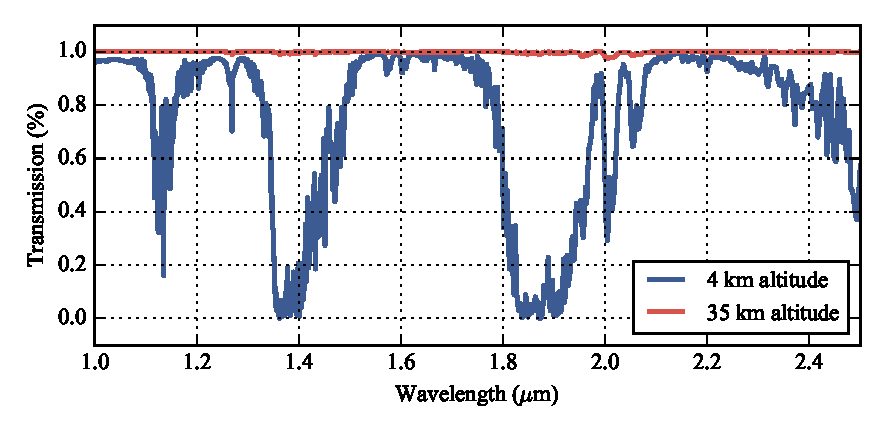
\includegraphics[width=\textwidth]{Figures/BETTII_atmo_transmission.pdf}
\vspace{-0.5cm}
\caption{Model atmospheric transmission, from \cite{Rizzo:2012jp}.}
\label{fig:trans}
\end{center}
\end{figure}

Due to the prioritization of the science channels, the NIR tracking channel is less advanced at the time of writing. Hence, we use estimates for the transmission and reflection efficiencies of the various components along the optical train. We estimate the efficiency of the major components: the mirrors (95\% reflective), the cryostat window (90\% transmissive), and the NIR/FIR dichroic (90\% transmissive), which transmits the NIR light. There is an additional filter just in front of the detector, which limits the bands from 1 to \SI{2.5}{\micro\meter}. The detectors are not responsive for longer wavelengths. The total amount of efficiency for this channel is expected to be on the order of $\epsilon = 20\%$. Using this, a \SI{1}{\jansky} source will correspond to a number of photons \Nph within a PSF at the detector:
\begin{align}
\Nph = \frac{\num{1e-26}}{h}\Area\times\FBW\times\epsilon\Tint \approx \num{8100},
\end{align}
where $\FBW \approx 0.67$ corresponds to the fractional bandwidth, and $h$ is the Planck constant. 

The detector is expected to have a read noise of $\sigRON = 18$~electrons r.m.s in up-the-ramp sampling, according the manufacturer specifications. Its frame rate changes throughout the acquire mode (see Chapter~\ref{chap:controls}), but the fastest mode will have a frame rate of $\sim\SI{50}{\hertz}$. Since the detector does not read destructively, saturation is an issue and needs to be addressed carefully - having to reset the pedestals to avoid saturation can complicate the software and might require a lot of tuning. Our calculations take into account a \SI{20}{\milli\second} integration time, a quantum efficiency of 70\%, and a \SI{0.6}{\arcsec\per\pixel} plate scale, which provides an effective background area $\beta = 0.43$ for a diffraction-limited PSF of diameter \ang{;;1.5} at \SI{1.5}{\micro\meter}. We consider that most of the photons will be spread on $1/\beta\approx~2.35$~pixels, so we expect about $\Nel\approx\num{3440}$~electrons per pixel from a \SI{1}{\jansky} source. A much more rigorous analysis is required once the efficiencies are measured.

For convenience, we express the \SNR of a source using its flux $S$ in electron per second:
\begin{align}
\SNR = \frac{S}{\sqrt{S + \beta(B + \sigRON^2)}},
\end{align}
where $B$ is the number of electrons per pixel from the background. In our case, we calculate $B\approx 2.4$~electrons, which is negligible compared to the read noise, so we will ignore this term in the future.

The required flux density for a given \SNR is then found by solving the previous equation for $S$:
\begin{align}
S\units{\si{\jansky}} = \frac{\SNR^2 + \sqrt{\SNR^4 + 4\SNR^2\beta\sigRON^2}}{2\Nel}.
\end{align}

For a $\SNR=10$, this corresponds to $\sim\SI{0.13}{\jansky}$, or $\sim$~9.66~H~magnitude.  For our first flight, all of our primary science targets have a star at least as bright within our field of view, which is usually embedded in the cluster itself.

\section{Targets}

The primary science targets for BETTII have fluxes that are above the spectral sensitivities from Table~\ref{tab:BETTIIsensitivity}, with a bright NIR guide star nearby. In addition, in order to correctly know the \OPD, we need sets of bright calibrator targets which provide high-\SNR fringes in one single scan of the delay line.

The science targets need to be available during our launch window, and preferably cover a large range of projected angles (so we can study the source at multiple angles to retrieve more of the spatial distribution). For this reason, we favor circumpolar sources, since they are the ones which change orientation at the fastest pace.


\subsection{Calibrators}

Calibrators ideally need to be point sources $\gg\SI{100}\Smin$~\si{\jansky} in our FIR bands, and it is not straightforward to identify which astronomical sources exist that would provide this kind of flux density. The planets of the solar system and their moons are usually bright enough, but they are often resolved by our instrument, which dramatically reduce their interferometric contrast. For example, we estimate the Uranus is $>\SI{1000}{\jansky}$, but because it is so resolved, the actual fringe contrast if very small, hence drastically reducing the \SNR. Nearby, bright A stars such as Alpha Boo are most likely point sources, but are usually not as bright as we would want, especially not in Band 2 since they are essentially thermal sources with temperatures of thousands of Kelvin. It is possible to use actual science sources as calibrators, but of course it is unknown whether or not they actually are extended (this is the purpose of a mission like BETTII!). 

We find that bright asteroids such as Ceres, Pallas and Vesta are the best candidates for bright calibrators (respectively $> 320, 150 and 120$~Jy). In addition, because of their albedo, they also reflect the sunlight so they would also be suitable for the tracking channels (e.g. Ceres has Hmag$\sim$3. Their only disadvantage is that they are not inertial targets - this complicates the pointing control system as their expected position moves across the sky, which requires the payload to have accurate timing capabilities to know where the object is at a given time.

\begin{figure}[!h]
	\centering
	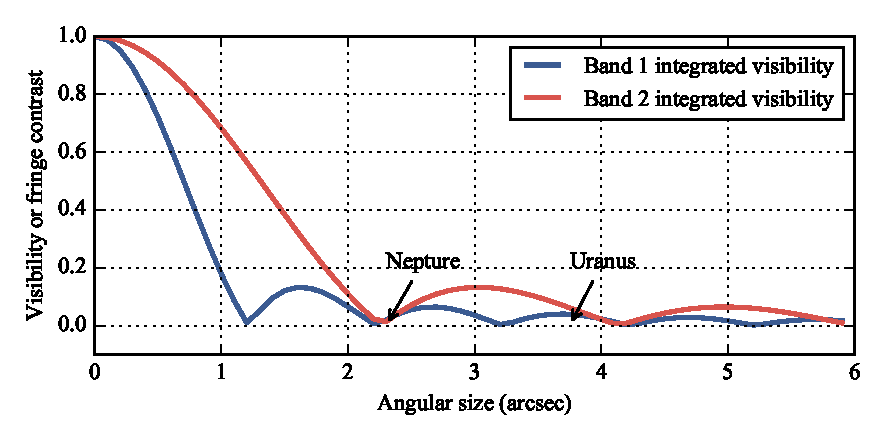
\includegraphics[width=\textwidth]{Figures/Visibilities.pdf}
	\caption[Visibilities of calibrators]{Visibilities of calibrators.}
	\label{fig:Visibilities}
    \end{figure}


\subsection{Science targets}
For our first flight, our science target list will be primarily composed of sources we have already observed with SOFIA FORCAST. In our source list, our best BETTII candidates are the sources which are bright at \SI{37}{\um}, have a large spectral index, appear point-like, are up in the sky at night during our flight, and are preferably circumpolar. 

\begin{table}[ht!]
\begin{center}
\caption{BETTII Targets}
\label{tab:BETTIITargets}
\vspace{-0.5cm}
\begin{longtable}{ccP{4cm}}
\toprule										
	Cluster	&	Coordinates	&	Fraction of night time between 15-\SI{75}{\degree} elevation		\\	
\midrule										
	S140	&	 22h19m23s +63d18m44s 	&	100.0	\%	\\		
	Cepheus~A	&	 22h56m10s +62d03m26s 	&	100.0	\%	\\	
	NGC~7129	&	 06h41m07s +09d33m35s 	&	100.0	\%	\\
	IRAS~20050+2720	&	 20h07m05s +27d28m51s 	&	50.0	\%	\\
\bottomrule										
\end{longtable}
\end{center}
\end{table}			

Table~\ref{tab:BETTIITargets} gives a list of such sources, and includes the fraction of time that the target spends above 10 degrees elevation and below \SI{75}{\degree} during the planned observing night of September 15, 2016. In addition, Fig.~\ref{fig:Targets} shows the tracks in the sky. The circumpolar targets S140, Cepheus~A and NGC~7129 are available for the most time. All are located well in the East at the beginning of the night, which means we can point towards them as the Sun sets in the West. Note that when the source is at low elevations, we could experience a substantial amount of additional atmospheric noise since the line of sight sees more airmass.

\begin{figure}[!h]
	\centering
	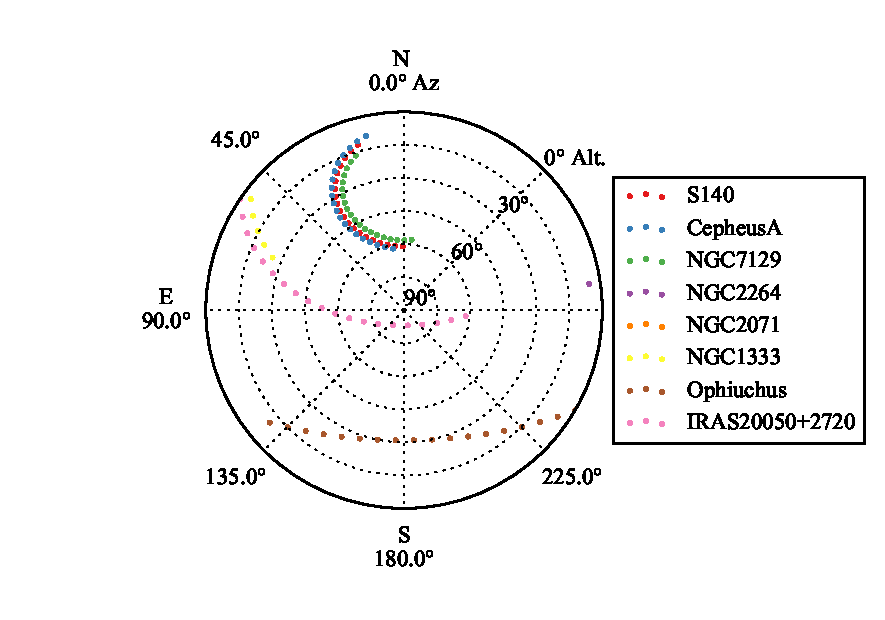
\includegraphics[width=\textwidth]{Figures/TargetPlot.pdf}
	\caption[Targets]{Polar plot showing the tracks of our targets in the night sky, between 8pm on Sept 15th and 6am on Sept 16th. The coordinates represent the local azimuth (with respect to North) and elevation, which is \SI{0}{\degree} at the horizon. Note that NGC~2071 and NGC~2264 cannot be observed at night in this period of the year.}
	\label{fig:Targets}
    \end{figure}
